% !TEX encoding = UTF-8
% !TEX TS-program = pdflatex
% !TEX root = ../Appunti.tex

\section{Introduzione}

In seguito si considera un modello di \textit{gas perfetto} per illustrare alcune delle affermazioni generali fatte.

\begin{defn}[Gas perfetto]
	Un \textit{gas perfetto} è un insieme di particelle (o, generalizzando, strutture elementari) \textit{non interagenti}.
\end{defn}

Per rendere il sistema \textit{non integrabile}, e quindi \textit{ergodico}, si deve però assumere che ci sia qualche modo per far scambiare impulso fra le particelle, e quindi farle interagire. Si può pensare ad un interazione mediata dalle pareti della scatola che contiene il gas.

\paragraph{Osservabili macroscopiche} A livello microscopico il sistema è quindi caratterizzato dall'Hamiltoniano di singola particella, e non c'è altro da aggiungere. Si vuole però caratterizzare il sistema nel suo insieme attraverso delle \textit{osservabili macroscopiche} e trovare le relazioni fra esse: si vuole trovare \textit{l'equazione di stato} del sistema complessivo.

Si vuole quindi indagare a livello microscopico l'origine di concetti macroscopici quali: \textit{entropia}, \textit{irreversibilità} e \textit{equilibrio}.

\subsection{Principi della Meccanica Statistica}
Per colmare il salto che separa la descrizione \textit{microscopica} dalle proprietà \textit{macroscopiche} del sistema la Meccanica Statistica di equilibrio pone essenzialmente due principi:

\begin{description}
	\item[Perdita di memoria:] all'equilibrio, che si suppone sempre raggiunto da un sistema dopo un tempo sufficientemente lungo (rispetto alle scale temporali delle interazioni microscopiche), il \textit{macrostato} del sistema è indipendente dalle condizioni iniziali.
	\item[Equiprobabilità a priori:] all'equilibrio ogni possibile \textit{microstato} è equiprobabile. La disponibilità di un data microstato dipende dai vincoli che deve soddisfare il sistema (es.: conservazione dell'energia).
\end{description}

\subsubsection{Equilibrio}

Si è parlato di \textit{equilibrio}, senza specificare cosa si intenda per esso. Non è una questione banale, ma a questo livello se ne può dare una definizione approssimativa.

\begin{defn}[Equilibrio]
	\label{def:eq}
	Si dice che un sistema macroscopico è all'\textit{equilibrio} quando tutte le osservabili macroscopiche sono \textit{stazionarie}, cioè non evolvono nel tempo.
\end{defn}

La \cref{def:eq} è approssimativa in quanto si considereranno in seguito trasformazioni fra stati di equilibrio.
\`E però una buona definizione se si specifica che la scala temporale su cui va valutata la stazionarietà è \textit{mesoscopica}: per tempo \textit{microscopici} il sistema evolve secondo la dinamica data dalle singole interazioni, mentre a livello \textit{macroscopico} l'evoluzione è data dalla trasformazione considerata.

Infatti per mantenere la condizione di equilibrio la scala microscopica e quella macroscopica sono separate da diversi ordini di grandezza, per cui è possibile la verifica della stazionarietà delle osservabili su scale intermedie, che vanno però considerate come nettamente distinte dalle altre (si può pensare a tre stati diversi, analogamente all'elettronica digitale in confronto alla natura analogica dei segnali).

\paragraph{Sulla natura dei principi fisici} \`E importante tenere presente che le due assunzioni fatte sono \textit{principi}, quindi non necessariamente verificati per ogni sistema fisico, ma sperimentalmente veri per un buon numero di sistemi e assunti per tutti gli altri.

A differenza di altri principi, che connettono l'astrazione teorica al mondo fisico, per natura stessa della meccanica statistica questi connettono due branche della teoria, quella microscopica e quella macroscopica, per cui è possibile che queste assunzioni siano false a livello formale per alcune classi di sistemi. Questo è il caso dei sistemi \textit{integrabili} (e quindi \textit{non ergodici}) in meccanica classica, ed è il caso di quasi tutti i sistemi quantistici (in cui la situazione è molto più sottile).

\'E sufficiente però considerare che questi sistemi sono pochi nel caso classico, mentre nel caso quantistico il problema si aggira in un altro modo, per cui i principi considerati consentono la descrizione di una classe enorme di sistemi (la quasi totalità).

\subsection{Entropia}
\label{sec:entro}

Si supponga che il sistema abbia $\Gamma$ possibili microstati, con $\Gamma \equiv \Gamma(E,N,V)$, cioè una funzione del volume, dell'energia e del numero totale dei componenti (d'ora in avanti \textit{particelle}) del sistema.

\begin{defn}[Entropia, microscopica]
	L'\textit{entropia} di un sistema è definita in base alle proprietà microscopiche di un sistema come:
	\begin{equation*}
	S = k \log\Gamma
	\end{equation*}
\end{defn}

In questo modo anche l'entropia è una funzione di volume, energia e numero di particelle del sistema $S \equiv S(E,N,V)$.

Invertendo l'entropia come funzione dell'energia si ottiene $E(S,N,V)$, e da questa espressione si possono studiare le variazioni dell'energia totale.

\begin{equation*}
	\dd E = \left(\frac{\partial E}{\partial S}\right)_{N,V} \dd S + \left(\frac{\partial E}{\partial V}\right)_{S,N} \dd V + \left(\frac{\partial E}{\partial N}\right)_{S,V} \dd N
\end{equation*}

\begin{note}[Invertibilità di $S(E,N,V)$]
	\'E sempre possibile invertire l'entropia in funzione dell'energia a $V$ e $N$ fissati, infatti se non c'è un limite superiore per l'energia di singola particella il numero di microstati sarà una funzione crescente dell'energia, e quindi anche l'entropia.
\end{note}

\paragraph{Osservabili intensive} Le osservabili estensive caratteristiche di un sistema macroscopico $E, N, V$ sono state definite in modo naturale a partire dalle caratteristiche microscopiche.

A questo punto si possono definire le osservabili intensive dalle variazioni dell'energia, distinguendo le varie sorgenti.

\begin{defn}[Osservabili Intensive]
	\label{def:ossint}
	Si definisce \textit{temperatura:}
	\begin{equation*}
	T = \left(\frac{\partial E}{\partial S}\right)_{N,V}
	\end{equation*}
	
	Si definisce \textit{pressione:}
	\begin{equation*}
	P = - \left(\frac{\partial E}{\partial V}\right)_{S,N}
	\end{equation*}
	
	Si definisce \textit{potenziale chimico:}
	\begin{equation*}
	\mu = \left(\frac{\partial E}{\partial N}\right)_{S,V}
	\end{equation*}
\end{defn}

Le definizioni che si sono date sono del tutto \textit{formali}, a priori senza alcun senso fisico alle spalle. Si esamina quindi una di queste (la temperatura) per capire la corrispondenza della definizione a un concetto fisico.

\paragraph{Temperatura} Il concetto fisico di temperatura è dato dal \textit{principio zero} della termodinamica: essa è una caratteristica del sistema che ne descrive l'equilibrio termico rispetto ad altri sistemi. La temperatura è quindi un numero reale:
\begin{itemize}
	\item condiviso per sistemi fra loro all'equilibrio;
	\item per sistemi non in equilibrio indica il verso in cui fluisce il calore.
\end{itemize}

Quando due sistemi, con numero di microstati $\Gamma_1$ e $\Gamma_2$, sono separati, il numero di microstati totale sarà $\Gamma_1\Gamma_2$.
Quando i sistemi sono posti in contatto, a $V$ e $N$ fissati per ciascuno, tutto ciò che può succedere macroscopicamente è che una parte dell'energia di uno fluisca nell'altro, e per la monotonicità dell'entropia quindi se aumenta $S_1$ allora diminuirà $S_2$ e viceversa.

Se i sistemi sono all'equilibrio l'entropia totale è allora in un massimo, altrimenti aumenterebbe tramite scambio di energia. Inoltre anche l'energia totale è conservata, per cui:

\begin{align*}
&\begin{rcases*}
\delta(E_1 + E_2) = 0 \\
\delta E_i = T_i \delta S_i
\end{rcases*}
\implies T_1 \delta S_1 + T_2 \delta S_2 = 0 \\
&\delta(S_1 + S_2) = 0
\end{align*}

\noindent Da cui si ottiene facilmente $T_1 = T_2$.

Si può verificare anche l'affermazione sul verso del flusso di energia (calore): sia $T_1 < T_2$, l'energia è sempre conservata, inoltre si considera che l'entropia totale può solo aumentare:

\begin{align*}
&\begin{rcases*}
\delta(E_1 + E_2) = 0 \\
\delta E_i = T_i \delta S_i
\end{rcases*}
\implies T_1 \delta S_1 + T_2 \delta S_2 = 0 \implies \implies \delta S_1 = - \frac{T_2}{T_1} \delta S_2\\
& \delta(S_1 + S_2) \geq 0 \implies \delta S_1 \geq - \delta S_2
\end{align*}

Da cui si ottiene:

\begin{equation*}
- \frac{T_2}{T_1} \delta S_2 \geq - \delta S_2 \implies (1 - \frac{T_2}{T_1}) \delta S_2 \geq 0 \implies \delta S_2 \leq 0
\end{equation*}

E per la monotonicità dell'entropia si ha anche $\delta E_2 \leq 0$, che corrisponde a quanto atteso.

\paragraph{Equazione di stato} A questo punto si è in grado di calcolare, astrattamente, l'\textit{l'equazione di stato}, eliminando l'entropia dalle due equazioni:

\begin{align*}
	&T(S,V,N) = \left(\frac{\partial E}{\partial S}\right)_{N,V} \\
	&P(S,V,N) = - \left(\frac{\partial E}{\partial V}\right)_{S,N}
\end{align*}

\subsection{Precisazioni teoriche sui fondamenti}
\label{sec:teorpipterm}
Anche se le temperatura di due sistemi è la stessa l'operazione di metterli a contatto non è senza conseguenze: si perde traccia dell'energia esatta di ognuno dei due sistemi, mantenendo l'informazione su quella totale.

Per cui si pongono due questioni:
\begin{itemize}
	\item quanta incertezza viene introdotta?
	\item negli argomenti usati precedentemente nello studio della temperatura, funziona tutto bene anche avendo perso traccia delle singole energie nel contatto termico?
\end{itemize}

La risposta alla prima domanda è: sostanzialmente poca, ed è per questo che la meccanica statistica funziona bene (si veda la \cref{sec:fluct}, per una trattazione più estesa).

La risposta alla seconda domanda è che non ci serve sapere quantitativamente l'energia, ma che è sufficiente sapere che il sistema è isolato e la sua energia è fissata.
\newline

C'è un punto ancora più sottile: oltre all'incertezza termodinamica sull'energia, se consentiamo le transizioni fra microstati a livello quantistico non siamo in uno stato stazionario, ma in stati con tempo di vita finito, e quindi vi è un'incertezza del tutto quantistica sulla loro energia.

Comunque se il numero di particelle è abbastanza grande questa incertezza non è rilevante: $\Gamma \sim 10^N$, per cui se anche l'errore sul conteggio degli stati fosse dell'ordine di $ N $ l'errore sul logaritmo (cioè sull'entropia) diventa irrisorio per grandi $ N $.

\paragraph{Descrizione canonica} Si può però rinunciare alla descrizione \textit{microcanonica} (energia fissata, vedi \cref{sec:statmech}) e decidere di considerare un piccolo sottosistema di un grande sistema isolato: per esso non sarà fissata l'energia, ma la temperatura, attraverso il contatto col resto del sistema che fungerà da \textit{bagno termico}.

L'energia del sistema quindi sarà libera di fluttuare, ma la descrizione si sposterà sulla \textit{densità di stati}, che non è soggetta a incertezza quantistica.

\begin{note}[Legge di dispersione]
	La \textit{densità di stati} tipicamente è determinata dal seguente procedimento:
	\begin{itemize}
		\item si assume che sia piatta sullo spazio delle fasi accessibile;
		\item si trasforma in una funzione dell'energia, una volta nota l'energia come funzione degli impulsi e delle poszioni.
	\end{itemize}
	Quest'ultima è a volte nota come \textit{legge di dispersione}.
\end{note}

\subparagraph{Fluttuazioni} \`E importante distinguere fra due tipi di fluttuazioni:
\begin{description}
	\item[fluttuazioni microscopiche:] si è detto che un sistema in equilibrio esplora tutti i microstati accessibili \textit{ergodicamente}, ma questo tipo di fluttuazioni fra microstati non sono fluttuazioni dell'equilibrio: l'equilibrio ha origine proprio da una media su queste transizioni;
	\item[fluttuazioni macroscopiche:] quando si è introdotto l'approccio \textit{canonico} si è inserita la possibilità che l'energia non fosse fissata, ma fluttuasse; queste fluttuazioni sono di tipo macroscopico, perché al livello microscopico descritto prima tanto il microcanonico quanto il canonico fluttuano.
\end{description}

% quest'ultima parte sulle fluttuazioni va rivista graficamente e dal punto di vista dell'italiano.

\section{Termodinamica}
\label{sec:termod}


\subsection{I principi della termodinamica}
La \textit{termodinamica} è fondamentalmente un sistema logico basato su quattro assiomi.

\paragraph{Principio zero} Il principio zero è stato già citato e discusso nella \cref{sec:teorpipterm}, esso caratterizza la relazione di equilibrio termico fra sistemi. Si riporta lo stesso un enunciato conciso:

\begin{defn}[Principio zero della termodinamica]
	La relazione di equilibrio termico è transitivi, quindi è una relazione di equivalenza.
	
	Più esplicitamente: se A è in equilibrio con B e con C, allora B è in equilibrio con C.
\end{defn}

\begin{note}
	C'è da fare attenzione anche in questo caso all'applicabilità fisica di questo principio: la verifica dell'equilbrio termico è effettuata mediante contatto termico, per cui per stabilire che due corpi non sono in equilibrio è necessario veder fluire calore.
	
	Se il calore che fluisce non è poco due corpi non in equilibrio potrebbero diventarlo. Cioè: la verifica dell'equilibrio fra due corpi può alterare la situazione iniziale, anzi, in generale \textbf{deve} farlo.
	
	Per aggirare questo problema ci si può servire di corpi sufficientemente piccoli di test (detti \textit{termometri}) che possono mediare il processo di verifica della situazione di equilibrio senza alterare apprezzabilmente lo stato dei corpi da testare, ed è in questo senso che va inteso il principio zero.
\end{note}

\paragraph{Primo principio} Il primo principio asserisce la \textit{conservazione dell'energia}: esso, macroscopicamente, corrisponde all'istituzione stessa di una quantità, detta energia, che si conservi in sistemi isolati.

\begin{defn}[Primo principio della termodinamica]
	L'energia è una quantità conservata per sistemi isolati.
	
	Più esplicitamente: se l'energia interna a un sottosistema del sistema isolato globale (da qui in poi detto \textit{universo}) non è conservata, essa è stata scambiata con altre parti dell'universo. Lo scambio di energia può assumere due forme: lavoro meccanico o calore.
	
	\begin{equation*}
		\dd E = \dd Q + \dd W
	\end{equation*}
	
	$Q$ è il calore assorbito dal sottosistema, mentre $W$ è il lavoro fatto sul sottosistema.
\end{defn}

\noindent Si noti che il lavoro meccanico corrisponde ad un trasporto di energia \textit{macroscopico}, mentre il calore è essenzialmente un trasporto di energia \textit{microscopico}. Questa è la principale differenza tra i due.

Per il \textit{gas perfetto} si può legare il lavoro alla variazione delle osservabili macroscopiche:

\begin{equation*}
\dd W = \mathcal{F} \dd x = \frac{\mathcal{F}}{A} (A\dd x) = - P \dd V
\end{equation*}

\noindent In generale è possibile identificare il lavoro, nell'ambito della meccanica lagrangiana, fermandosi alla prima uguaglianza e considerando come $\dd x$ gli spostamenti generalizzati e com $ \mathcal{F} $ le forze generalizzate corrispondenti (bisognerà inoltre sommare su tutti i possibili contributi).
\newline

Si ottiene quindi che:
\begin{equation*}
	\left(\frac{\partial E}{\partial V}\right)_Q = - P
\end{equation*}

\noindent Che può essere confrontato con la definizione data nella \cref{sec:entro}.

Questo è legato al fatto che una trasformazione \textit{isoentropica} avviene senza scambio di calore, infatti variando in modo sufficientemente lento il volume per il \textit{teorema adiabatico} i microstati cambieranno, ma ci sarà una corrispondenza uno a uno fra vecchi e nuovi, quindi il loro numero è fissato.

Queste ultime affermazioni in realtà sono tutte nell'ottica della meccanica statistica, perché a livello termodinamico l'entropia è definita nell'ambito del \textit{secondo principio}, che non è stato ancora esposto.

\paragraph{Secondo principio} Il secondo principio è enunciato nel modo più termodinamicamente corretto nelle forme di \textit{Kelvin} e di \textit{Clausius}, ben note e reperibili. Esse consentono la dimostrazione del teorema di \textit{Carnot}, e conseguentemente di quello di \textit{Clausius}, che consente di definire l'entropia.

Si sceglie allora di assumere noto il teorema di \textit{Clausius}, definendo l'entropia, e servendosi di essa per enunciare il secondo principio, ma deve essere noto che questo non è realmente possibile in termodinamica, in quanto il secondo principio è logicamente precedente alla definizione stessa di entropia.

\begin{defn}[Entropia]
	La variazione di entropia fra uno stato A e uno stato B è:
	\begin{equation*}
	\Delta S = \int_{A \rightarrow B} \frac{\dd Q}{T}
	\end{equation*}
	dove l'integrazione è effettuata su un cammino costituito da una trasformazione \textit{reversibile}.
	
	L'entropia è quindi definita così a meno di una costante, che fissa il valore dell'entropia per un certo stato.
\end{defn}

\noindent E dunque:

\begin{defn}[Secondo principio della termodinamica]
	L'entropia di un sistema isolato fuori equilibrio tende ad aumentare.
\end{defn}

\noindent Gli stati di equilibrio sono quindi caratterizzati come massimi dell'entropia.

\paragraph{Terzo principio} Il terzo principio si colloca ai margini della termodinamica, e più che farne parte ne specifica i limiti. Infatti esso afferma che:

\begin{defn}[Terzo principio della termodinamica]
	L'entropia a temperatura nulla (zero assoluto) è nulla.
\end{defn}

\noindent che in modo equivalente può essere inteso come: \textit{la temperatura nulla non è raggiungibile da processi termodinamici.}

\subsection{Grandezze termodinamiche}
\label{sec:thermquant}

Vi sono quattro variabili termodinamiche principali, non indipendenti:

\begin{equation*}
\begin{matrix}
S	&	V \\
T	&	P \\
\end{matrix}
\end{equation*}

\noindent Organizzate nel modo seguente:
\begin{itemize}
	\item la prima riga sono estensive;
	\item la seconda riga intensive;
	\item le variabili appartenenti alla stessa colonna sono coniugate.
\end{itemize}

\noindent Le variabili coniugate compaiono a coppie nell'espressione dell'energia. Ogni variabile termodinamica può essere espressa come funzione della variabile coniugata e di una delle altre due (si verifica a partire dalle espressioni date nella \cref{def:ossint}).

Perciò è sempre possibile scegliere una coppia di variabili, non coniugate, come \textit{indipendenti}, le altre due saranno quindi \textit{dipendenti} e ottenibili come funzioni delle prime.
\newline

Le variabili termodinamiche scelte come \textit{dipendenti} possono essere ricavate da un singolo \textit{potenziale termodinamico}, se le variabili indipendenti scelte sono le variabili \textit{proprie} del potenziale.

I potenziali termodinamici sono ottenuti come opportune trasformate di Legendre dell'energia, si passa quindi ad illustrarli.

\paragraph{Energia E} Le sue variabili proprie sono $S$ e $V$. L'espressione del suo differenziale è:

\begin{equation*}
\dd E = T \dd S - P \dd V
\end{equation*}

\paragraph{Energia libera F} Le sue variabili proprie sono $T$ e $V$. La sua espressione in funzione dell'energia $E$ è:

\begin{equation*}
F = E - T S
\end{equation*}

E dunque l'espressione del suo differenziale è:

\begin{equation*}
\dd F = - S \dd T - P \dd V
\end{equation*}

\begin{note}
	Le variabili proprie dell'energia libera sono particolarmente comode (il motivo è per lo più che non contengono l'entropia), per cui essa è decisamente utile ai fini del calcolo dell'equazione di stato, cioè $ P(V,T) $ (un altro motivo è che si esprime in modo semplice in termini della \textit{funzione di partizione}, vedi \cref{sec:statmech}).
\end{note}

\paragraph{Energia libera di Gibbs G }Le sue variabili proprie sono $T$ e $P$. La sua espressione in funzione dell'energia $E$ è:

\begin{equation*}
G = E - T S + P V
\end{equation*}

E dunque l'espressione del suo differenziale è:

\begin{equation*}
\dd G = - S \dd T + V \dd P
\end{equation*}

\begin{note}
	Anche questo potenziale ha una sua utilità specifica: esso è espresso in funzione delle variabili \textit{intensive}, questo lo rende particolarmente per caratterizzare alcune situazioni (es: \textit{transizioni di fase}).
\end{note}


\paragraph{Entalpia H}Le sue variabili proprie sono $S$ e $P$. La sua espressione in funzione dell'energia $E$ è:

\begin{equation*}
H = E + P V
\end{equation*}

E dunque l'espressione del suo differenziale è:

\begin{equation*}
\dd H = T \dd S + V \dd P
\end{equation*}

Si nota che l'entalpia ha una proprietà per cui in inglese è chiamata anche \textit{heat function}, ed è:

\begin{equation*}
\dd H)_P = T \dd S)_P = \dd Q)_p
\end{equation*}

\subsubsection{Relazioni di Maxwell}
Applicando il \textit{teorema di Schwarz} (di cui supponiamo sempre verificate le ipotesi, lontano da punti critici) si ha la commutazione delle derivate seconde, e applicando questo risultato ai vari potenziali termodinamici si ottengono le cosiddette \textit{relazioni di Maxwell}.

Si riporta solo il caso dell'energia libera a titolo di esempio:

\begin{equation*}
\left(\frac{\partial P}{\partial T}\right)_V = \frac{\partial}{\partial T} \left(- \left(\frac{\partial F}{\partial V}\right)_T\right)_V = \frac{\partial}{\partial V} \left(- \left(\frac{\partial F}{\partial T}\right)_V\right)_T = \left(\frac{\partial S}{\partial V}\right)_T
\end{equation*}

\`E noto un diagramma che riassume le proprietà dei potenziali termodinamici, cioè le variabili proprie e le relazioni di Maxwell, ed è considerato un utile strumento mnemonico (\cref{fig:maxrel}).

\begin{figure}[t]
	\centering
	\input{MaxRel.pdf_tex}
	\caption{Diagramma illustrativo delle relazioni fra potenziali termodinamici (noto anche come \textit{diagramma di koenig} )}
	\label{fig:maxrel}
\end{figure}

\subsubsection{Numero di particelle}
Fino ad adesso si è considerato costante il numero di particelle, ma in base alla scelta che si fa del sottosistema anche esso può essere variabile: non è necessario che un sottosistema sia identificato dalla scelta di alcune particelle, che in generale è impossibile da effettuare (vedi \cref{secidpart}), ma potrebbe essere descritto da altre proprietà (es: il volume che occupa, un certo insieme di stati, \dots).

Perciò, coerentemente con la \cref{def:ossint}, si può scrivere:

\begin{equation*}
\dd E = T \dd S - P \dd V + \mu \dd N
\end{equation*}

\noindent Da questa inoltre risultano le espressioni degli altri potenziali termodinamici, ottenute differenziando le opportune trasformate di Legendre.

\begin{note}
	Un'importante osservazione è che le variazioni dei potenziali termodinamici rispetto a qualunque nuova osservabile, tenendo costanti le variabili proprie, sono tutte uguali, infatti:
	
	\begin{equation*}
	\mu \delta N = (\delta E)_{S, V} = (\delta F)_{T,V} = (\delta G)_{T,P} = (\delta H)_{S,P}
	\end{equation*}
\end{note}

Inoltre si noti che $E$ è una grandezza estensiva, le cui variabili proprie sono anch'esse estensive; sfruttando questa proprietà si ha che scalando di una quantià $\lambda$ il sistema\footnote{Si immagini di frazionare in parti il sistema, se il sistema è sufficientemente grande posso coprire tutto $\mathbb{Q}^+$, e passando al limite $\mathbb{R}^+$.}:

\begin{align*}
& \dd (\lambda E) = T \dd (\lambda S) - P \dd (\lambda V) + \mu \dd (\lambda N) \implies\\ 
& \qquad \implies E \dd \lambda + \lambda \dd E  = T (S \dd \lambda + \lambda \dd S) - P (V \dd \lambda + \lambda \dd V) + \mu (N\dd \lambda + \lambda \dd N)
\end{align*}

Raccogliendo $\lambda$ e $\dd lambda$, e considerando che poiché $\lambda$ è arbitrario le due identità risultanti devono essere soddisfatte separatamente, si ottiene l'equazione di Eulero:

\begin{equation*}
E = TS - PV + \mu N
\end{equation*}

Da cui si ottiene l'espressione per la variazione del potenziale chimico:

\begin{equation*}
\dd \mu = - \frac{S}{N} \dd T + \frac{V}{N} \dd P
\end{equation*}

L'equazione di Eulero per l'energia implica che anche gli altri potenziali termodinamici possano avere una forma simile. In particolare:

\begin{equation*}
G = \mu N
\end{equation*}

\paragraph{Gran Potenziale $\Omega$} Si può definire un ulteriore potenziale termodinamico, invertendo le nuove variabili $N \rightarrow \mu$. Le sue variabili proprie sono $T$, $V$ e $\mu$. La sua espressione in funzione dell'energia $E$ è:

\begin{equation*}
\Omega = F - \mu N = E - TS - \mu N
\end{equation*}

E dunque l'espressione del suo differenziale è:

\begin{equation*}
\dd \Omega = - S \dd T - P \dd V - N \dd \mu
\end{equation*}

Dall'equazione di Eulero si ricava:

\begin{equation*}
\Omega = - P V
\end{equation*}

\subsection{Variabili Magnetiche}
Lo studio del magnetismo in termodinamica è frequente, e la definizione di variabili magnetiche non è affatto dissimile dall'introduzione di pressione e volume per il gas perfetto come forza e spostamento \textit{generalizzati}.

Si nota solo che il ruolo di forza generalizzata in questo ambito è svolto dal campo magnetico $ H $, mentre lo spostamento generalizzato è $ \dd (M V) $ dove $M$ è la magnetizzazione del mezzo e $V$ è ancora il volume.

\subsection{Principio variazionale}
Il principio variazionale fondamentale in termodinamica è quello fissato dal \textit{secondo principio}: l'entropia per uno stato di equilibrio è massima.

Questo si riflette in una serie di principi variazionali ausiliari, dettati dalla possibilità di raggiungere l'equilibrio tenendo costanti alcune delle variabili termodinamiche.

\begin{align*}
	T, V, N = cost. \qquad \implies \qquad F = \text{minimum}\\
	T, P, N = cost. \qquad \implies \qquad G = \text{minimum}\\
	T, V, \mu = cost. \qquad \implies \qquad \Omega = \text{minimum}\\
\end{align*}

Si posson ottenere considerando il sottosistema che fluttua alla ricerca dell'equilibrio e il bagno termico, il cui stato di equilibrio non è influenzato dalle fluttuazioni del sottosistema. Perciò si ha:

\begin{equation*}
\begin{rcases*}
\begin{rcases*}
\dd E' = T \dd S' - \dd W'\\
\delta (E + E') = 0
\end{rcases*} \dd E + T \dd S' - \dd W' = 0\\
\delta (S + S') \geq 0
\end{rcases*}
\delta E \leq T \delta S + p \delta V
\end{equation*}

Dall'ultima espressione si ottiene facilmente l'enunciato per $F$, ponendo $\delta V = 0$ e $T \delta S = \delta (T S)$. Analogamente si può fare per gli altri due casi.

\subsection{Derivate termodinamiche}

Si è visto nella \cref{sec:thermquant} come le variabili termodinamiche possano essere ottenute come derivate prime dei potenziali termodinamici, che costituisce la prima definizione data di alcune di esse (\cref{def:ossint}).

Si consideri d'ora in avanti i potenziali termodinamici come le quantità termodinamiche \textit{massimamente integrate}, le altre grandezze termodinamiche saranno caratterizzate dall'essere ottenute a un qualche ordine di derivazione da esse.

Perciò, se le variabili stesse costituiscono il \textit{primo ordine di derivazione}, si prenderà in esame adesso il \textit{secondo ordine di derivazione}. Si è già parlato di esso nella \cref{sec:thermquant}, a proposito delle \textit{relazioni di Maxwell}; in quell'ambito si sono considerate solo le derivate seconde miste, passiamo quindi a considerare le altre.

\begin{defn}[Capacità termica]
	Si definisce \textit{capacità termica a volume costante} la quantità $C_V$:
	\begin{equation*}
	C_V = T \left(\frac{\partial S}{\partial T}\right)_V
	\end{equation*}
	Si definisce \textit{capacità termica a pressione costante} la quantità $C_P$:
	\begin{equation*}
	C_P = T \left(\frac{\partial S}{\partial T}\right)_P
	\end{equation*}
\end{defn}

\noindent La capacità termica quantifica la variazione di temperatura $\delta T$ in base allo scambio di calore $T \delta S$.

Per la capacità termica $C_V$ si nota la relazione:
\begin{equation*}
C_V = \left(\frac{\partial E}{\partial T}\right)_V
\end{equation*}

\noindent è però importante rendersi conto che la temperatura $T$ non è una delle variabili proprie dell'energia.

Per entrambe le capacità termiche si può esprimere però propriamente in funzione dei potenziali termodinamici con le variabili proprie adeguate:

\begin{align*}
C_V = T \left(\frac{\partial^2 F}{\partial T^2}\right)_V\\
C_P = T \left(\frac{\partial^2 G}{\partial T^2}\right)_P
\end{align*}

\noindent che giustifica il fatto che esse siano grandezze del \textit{secondo ordine} (d'ora in poi è omesso che si tratti di derivate).
\newline

Analogamente si possono definire le \textit{compressibilità}:

\begin{defn}[Compressibilità]
	Si definisce \textit{compressibilità isoterma} la quantità $K_T$:
	\begin{equation*}
	K_T = - \frac{1}{V} \left(\frac{\partial V}{\partial P}\right)_T
	\end{equation*}
	Si definisce \textit{compressibilità adiabatica} la quantità $K_S$:
	\begin{equation*}
	K_S = - \frac{1}{V} \left(\frac{\partial V}{\partial P}\right)_S
	\end{equation*}
\end{defn}

Anche in questo caso è possibile esprimere le compressibilità in funzione di opportune derivate seconde:

\begin{align*}
&K_T = - \frac{1}{V} \left(\frac{\partial^2 G}{\partial P^2}\right)_T\\
&K_S = - \frac{1}{V} \left(\frac{\partial^2 H}{\partial P^2}\right)_S = \left[ V \left(\frac{\partial^2 E}{\partial V^2}\right)_S \right]^{-1}
\end{align*}

\paragraph{Relazioni notevoli} Attraverso la definizione dei differenziali delle variabili termodinamiche si possono ottenere delle importanti relazioni fra le quantità appena definite.
Ad esempio, per le capacità termiche:
\begin{align*}
&\begin{rcases*}
\dd S = \left(\frac{\partial S}{\partial P}\right)_T \dd P + \left(\frac{\partial S}{\partial T}\right)_P \dd T\\
\left(\frac{\partial S}{\partial P}\right)_T = - \left(\frac{\partial V}{\partial T}\right)_P
\end{rcases*}
\qquad \frac{C_V}{T} = \left(\frac{\partial S}{\partial T}\right)_V = \left(\frac{\partial S}{\partial P}\right)_T \left(\frac{\partial P}{\partial T}\right)_V + \frac{C_P}{T} \implies\\
&\qquad \qquad \implies \frac{C_P - C_V}{T} = \left(\frac{\partial V}{\partial T}\right)_P \left(\frac{\partial P}{\partial T}\right)_V
\end{align*}

Da cui si ottiene infine, applicando \textit{chain rule}\footnote{\`E necessario notare che la relazione corretta, dimostrabile mediante l'uso di opportuni Jacobiani, è:
\begin{equation*}
	\left(\frac{\partial V}{\partial T}\right)_P \left(\frac{\partial T}{\partial P}\right)_V \left(\frac{\partial P}{\partial V}\right)_T = -1
\end{equation*}
}:

\begin{equation*}
C_P - C_V = T V K_T \left[\left(\frac{\partial P}{\partial T}\right)_V\right]^2 = \frac{T}{V K_T} \left[\left(\frac{\partial V}{\partial T}\right)_P\right]^2
\end{equation*}

\paragraph{Variabili magnetiche} Anche nel caso di variabili magnetiche le quantità definite dalle derivate seconde non miste sono rilevanti, e vengono chiamate \textit{suscettività.}

\begin{defn}[Suscettività]
	Si definisce \textit{suscettività isoterma} la quantità $K_T$:
	\begin{equation*}
	X_T = \left(\frac{\partial M}{\partial H}\right)_T
	\end{equation*}
	Si definisce \textit{suscettività adiabatica} la quantità $K_S$:
	\begin{equation*}
	X_S = \left(\frac{\partial M}{\partial H}\right)_S
	\end{equation*}
\end{defn}

E anche in questo caso si può ottenere una relazione simile a quella per $C_V$ e $C_T$ nel caso delle capacità termiche a magnetizzazione e campo costante, rispettivamente $C_M$ e $C_H$. 

\begin{equation*}
C_H - C_M = \frac{T V}{X_T} \left[\left(\frac{\partial M}{\partial T}\right)_H\right]^2
\end{equation*}

\subsubsection{Funzioni di risposta} Le quantità definite prima caratterizzano la risposta lineare del sistema agli stimoli esterni, per si ha la seguente definizione:

\begin{defn}[Funzioni di risposta]
	Le capacità, compressibilità e suscettività vengono definite collettivamente \textit{funzioni di risposta.}
\end{defn} 

\paragraph{Proprietà} Si mostrano ora alcune proprietà delle funzioni di risposta:
\begin{itemize}
	\item $K_T \geq 0$: si consideri un sistema isolato con $N,T$ e $V$ costanti, si ha quindi che il sistema tende a minimizzare l'energia libera $F$. Si consideri inoltre il sistema diviso in due parti.
	\begin{align*}
	\begin{rcases*}
	\dd V_1 + \dd V_2 = \dd V = 0\\
	\delta F \geq 0
	\end{rcases*}
		 \frac{\partial F}{\partial V_1} = \frac{\partial F_1}{\partial V_1} + \frac{\partial F_2}{\partial V_1} = \frac{\partial F_1}{\partial V_1} - \frac{\partial F_2}{\partial V_2} = 0
	\end{align*}
	dove si è usato solo che $F$ è in un punto stazionario, e si è trovato infine $P_1 = P_2$, che è intuitivo caratterizzi l'equilibrio meccanico (deriva dall'\textit{equilibrio delle forze}).
	
	Il fatto che $F$ sia in un minimo da un informazione ulteriore sulle derivate seconde:
	\begin{equation*}
	 \frac{\partial^2 F}{\partial V_1^2} =  \frac{\partial}{\partial V_1} (P_2 - P_1) =  -\frac{\partial P_1}{\partial V_1} -\frac{\partial P_2}{\partial V_2} \geq 0 \implies \frac{1}{V_1 K_{T_1}} + \frac{1}{V_2 K_{T_2}} \geq 0
	\end{equation*}
	Considerando le due parti del sistema composte dallo stesso numero di particelle, $N_1 = N_2$, si ottiene che, poiché si è dimostrato che la condizione di equilibrio impone che temperatura e pressione siano anch'esse le stesse (e quindi anche i volumi sono uguali per l'equazione di stato), si ha che $K_{T_1} = K_{T_2}$, da cui la tesi.
	\item $C_V \geq 0$: gli argomenti che si usano nella dimostrazione sono simili al caso precedente, per cui si mettono in luce solo le differenze:
	\begin{itemize}
		\item si considera un sistema con isolato, quindi con $E$ e $V$ costanti, anziché $T$ e $V$;
		\item si ha quindi che il principio variazionale da usare è direttamente quello per $S$, anziché la forma per $F$;
		\item si trova che all'equilibrio le temperature sono uguali, anziché le pressioni.
	\end{itemize}
	\item $C_P \geq 0$: si possono sviluppare argomenti analoghi per $C_P$, ma nella sezione precedente si è dimostrata una relazione notevole per la differenza delle capacità termiche, il cui membro di destra era sempre positivo, per cui: $C_P \geq C_V \geq 0$.
\end{itemize}

Si noti che le proprietà mostrate dovevano risultare vere già a livello concettuale, prima della dimostrazione formale:
\begin{description}
	\item[compressibilità] la positività della compressibilità è equivalente ad affermare che all'aumentare della pressione interna il corpo tenda ad espandersi;
	\item[capacità termica] la positività della capacità termica è equivalente ad affermare che ad un aumento di temperatura corrisponde un aumento di energia interna.
\end{description}

L'intuitività del secondo è minata dal fatto che il concetto di temperatura non è affatto intuitivo, ma piuttosto formale; si recupera in parte l'intuizione ricordando che la temperatura è quella quantità che caratterizza il verso del flusso di calore fra due corpi non all'equilibrio. Per cui il segno della capacità termica è stato \textit{scelto} quando si è scelto che il calore fluisse dal corpo a temperatura più alta verso quello a temperatura più bassa.

\subsection{Diagrammi di fase}

\subsubsection{Digressione sul concetto di fase}
La materia che stiamo considerando è composta da particelle, la cui struttura interna è fissata, ma la struttura che assume l'insieme di questi corpi può dipendere fortemente dalle osservabili macroscopiche. La possibilità di distinguere proprio a livello macroscopico queste tipologie di organizzazione determina il concetto di \textit{fase}.

La definizione del concetto di \textit{fase} non è affato banale, per cui si cita quella data dalla \href{http://www.treccani.it/enciclopedia/fase/#chimica-1}{Treccani}:

\begin{defn}[Fase]
	In un sistema eterogeneo si definiscono f. le parti omogenee, di uguale composizione chimica e di uguale stato fisico, separabili meccanicamente. Così, i gas che sono sempre completamente miscibili formano un’unica f.; i liquidi formano più f. quando sono fra loro non completamente miscibili; i solidi possono dare un illimitato numero di fasi. Più in generale, si chiama f. una qualsiasi porzione di un sistema fisico-chimico per la quale siano costanti tutti i parametri che la individuano chimicamente e fisicamente (pressione, temperatura, densità, entropia, costituzione chimica ecc.).
\end{defn}

Questa è una buona definizione a livello enciclopedico, forse un po' povera se confrontata col livello di formalità generale. La cosa importante è chiarire esplicitamente a livello concettuale cosa implica la nozione di fase, per cui si prova a caratterizzarla:

\begin{itemize}
	\item essa è chiaramente riferita ad una porzione estesa di materia, per cui è richiesta una certa coerenza fra le proprietà \textit{mesoscopiche} all'interno della regione spaziale considerata, al punto da poterle considerare uniformi; è importante considerare le proprietà mesoscopiche, perché:
	\begin{itemize}
		\item si vogliono considerare punti spazialmente diversi (le proprietà macroscopiche riguardano l'intero sistema, per cui non possono dipendere dal punto);
		\item non si stanno considerando le proprietà microscopiche, che invece variano drasticamente sulle scale tipiche delle singole particelle (si pensi agli atomi e i campi elettrici).
	\end{itemize}
	\item proprio per l'uniformità richiesta tale nozione implica un certo ordine, un certo tipo di organizzazione (o la sua assenza) che si ripete nei vari punti dello spazio; a posteriori, pensando ai vari tipi di fase noti, è chiaro il senso di questa affermazione. 
\end{itemize}

\subsubsection{Piano $P-T$}

La presenza delle varie fasi è ben visualizzabile nel piano $P-T$. La \cref{fig:phdiagr} illustra il caso tipico di un diagramma delle fasi.

\begin{wrapfigure}{R}{0.5\textwidth}
	\vspace{-30pt}
	\centering
	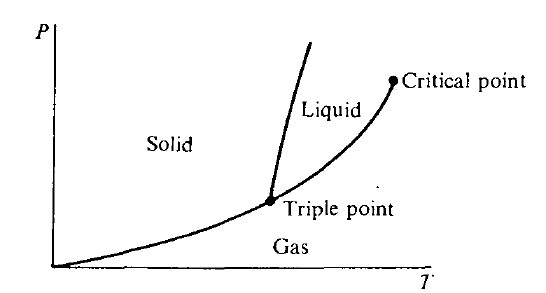
\includegraphics[width=0.5\textwidth]{Immagini/PhaseDiagram.png}
	\caption{}
	\label{fig:phdiagr}
	\vspace{-30pt}
\end{wrapfigure}

Ci sono varie osservazioni da fare:
\begin{itemize}
	\item la più importante è la scelta delle variabili $P-T$, esse sono variabili intensive, e il motivo è chiaro: se la \textit{fase} è caratterizzata dall'uniformità essa non potrà direttamente dipendere da proprietà estensive quali il volume, infatti raddoppiando il sistema (numero di particelle compreso) esso manterrà lo stesso tipo di ordine, sarà solo più grande;
	\item le linee marcate nel diagramma sono note come \textit{linee di coesistenza}, e in quei punti nel sistema sono presenti le due fasi contemporaneamente; essendo oggetti $1$-D sono individuati da una sola variabile, infatti fissata una fra pressione e temperatura l'altra è determinata dalla condizione di coesistenza;
\end{itemize}

\begin{itemize}
	\item il punto di intersezione fra le due linee di coesistenza è detto \textit{punto triplo}, in esso coesistono le tre fasi, ed è individuato da una esatta pressione e temperatura;
	\item la lineaa di coesistenza tra \textit{liquido} e \textit{gas} termina in un punto critico: questo implica che non si può realmente distinguere fra l'uno e l'altro, perché è possibile cambiare fase in modo continuo, aggirando tale punto\footnote{\`E però evidente che se il punto critico è piuttosto distante è abbastanza facile distinguere tra liquido e gas, perché potreste non essere praticamente possibile realizzare un percorso che aggiri il punto critico.}.
\end{itemize}

Si riporta inoltre un altro diagramma, relativo al piano $P-V$:

\begin{figure}[H]
	\centering
	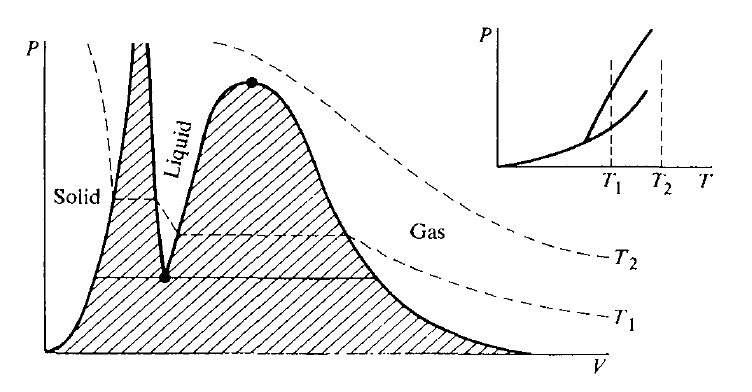
\includegraphics[width=0.7\textwidth]{Immagini/PhasePV.png}
	\caption{}
	\label{fig:phasepv}
\end{figure}

Ciò che si vuole evidenziare di esso è che la \textit{"traiettoria"} delle curve isoterme (tratteggiate in figura) nella regione tratteggiata (regione di coesistenza): esse coincidono con delle isobare, corentemente con quanto descritto a proposito delle curve di coesistenza.
Le variabili $P$ e $T$ non sono quindi sufficienti in questa regione a descrivere il sistema, poiché a $P$ e $T$ fissati sono possibili diversi valori di $V$.

Quello che sta accadendo è che $V$ descrive quanta parte del sistema è in una o in un'altra fase, poiché nella varie fasi cambia il \textit{volume specifico} $V/N$; per cui nella regione ad alto $V$ il sistema sarà prevalentemente nella fase ad alto volume specifico, e viceversa nella regione a basso $V$.

Ci sono altre cose interessanti da notare in questo grafico: la posizione del punto critico e quella del punto triplo, la \textit{separazione} tra solido e liquido, la transizione "diretta" da gas a solido. Si lascia al lettore lo studio di questa proprietà sul diagramma.

\subsubsection{Equazione di Clausius-Clapeyron}

Nella \cref{fig:phdiagr} si può inoltre notare come tutte le curve di coesistenza abbiano derivata sempre positiva. Questa è una proprietà frequente, ma non necessaria.

Il motivo è il seguente, e verrà verificato a posteriori: se l'entropia specifica e il volume specifico crescono in modo concorde da una fase all'altra la pendenza della curva sarà positiva, se discorde sarà negativa.

Intuitivamente ciò che succede è che ad alta temperatura sarà privilegiata la fase più entropica (ha un peso maggiore nell'energia libera di Gibbs) mentre ad alta pressione quella a più alta densità, quindi più basso volume specifico. Se una stessa fase soddisfa entrambi i requisiti allora la pendenza della curva sarà negativa, e la variazione discorde, viceversa nell'altro caso. 
\newline

Per ricavare il risultato precedente si consideri un sistema isolata, costituito da due sottosistemi, che condividono lo stesso volume e lo stesso insieme di particelle, e sono distinti dallo stato: ciascuno rappresenta una diversa fase.

Dalle condizioni di equilibrio ricavate precedentemente si ha $T_1 = T_2$ e $P_1 = P_2$. Un ulteriore condizione si ottiene considerando:
\begin{align*}
\begin{rcases*}
\dd N_1 + \dd N_2 = \dd V = 0\\
\delta F \geq 0
\end{rcases*}
\frac{\partial F}{\partial N_1} = \frac{\partial F_1}{\partial N_1} + \frac{\partial F_2}{\partial N_1} = \frac{\partial F_1}{\partial N_1} - \frac{\partial F_2}{\partial N_2} = 0
\end{align*}

\noindent Perciò $\mu_1 = \mu_2$.

Da questa uguaglianza si può ricavare un'equazione per $P$ e $T$:

\begin{equation*}
\mu_1 (P,T) = \mu_2 (P,T)
\end{equation*}

Per cui si può risolvere per una delle due variabili e ottenere l'equazione esplicita della curva (si noti che se le fasi che coesistono fossero tre ci sarebbe un'altra equazione da soddisfare, cioè l'uguaglianza con $\mu_3$, questo porterebbe ad individuare un unico punto, il punto triplo).

Per ricavarsi l'equazione della curva è quindi necessaria l'espressione esplicita del potenziale chimico in funzione delle due variabili indicate. Questa può essere ricavata da una teoria microscopica delle fasi.

Si può comunque ricavare un utile risultato dalla relazione di Gibbs-Duhem:

\begin{align*}
&\dd \mu_1 = \dd \mu_2 \implies -s_1 \dd T + v_1 \dd P = -s_2 \dd T + v_2 \dd P \implies \\
&\qquad \implies \derivative{ P_0}{T} = \frac{s_2 - s_1}{v_2 - v_1}
\end{align*}

\noindent dove si è usato $s = S/N$ e $v = V/N$, rispettivamente entropia e volume specifici.

In questo ambito si definisce inoltre il \textit{calore latente}:

\begin{defn}[Calore latente]
	\`E una grandezza $\lambda$ delle dimensioni di un'energia (un calore), che caratterizza le transizioni di fase discontinue, cioè quelle in cui è presente una differenza finita di entropia specifica tra le due fasi.
	\begin{equation*}
		\lambda = T(s_2 - s_1) = T \Delta s
	\end{equation*} 
\end{defn}

Alla luce di questa nuova definizione l'equazione di Clausius-Clapeyron è espressa in modo naturale come:

\begin{equation*}
\derivative{ P_0}{T} = \frac{\lambda}{T(v_2 - v_1)}
\end{equation*}

\section{Meccanica Statistica}
\label{sec:statmech}

Il compito della meccanica statistica è principalmente \textit{contare il numero di stati possibili} per un dato macrostato, cioè trovare $\Gamma(E,V,N)$, come indicato nella \cref{sec:entro}.

Da esso infatti sarà possibile trovare l'espressione per l'entropia, e invertendo ques'ultima si avrà l'energia in funzione delle sue variabili proprie, che determina in modo completo la dinamica macroscopica.

In reltà non è conveniente cercare di ottenere $E(S,V,N)$, perché l'entropia non è una variabile così naturale, specie dal punto di vista sperimentale. Si cercherà invece di ottenere la funzione $ F(T,V,N) $, oppure $ \Omega(T,V,\mu) $, le cui variabili proprie risultano molto più intuitive (si ribadisce che l'equazione per la pressione a partire da $ F $ è direttamente l'equazione di stato).

\subsubsection{Derivazione}
Poiché si è interessati a un sistema in cui è fissata la sola temperatura $ T $, o essa e il potenziale chimico $ \mu $, anziché l'energia, si ricorrerà alla descrizione \textit{canonica} introdotta nella \cref{sec:teorpipterm}, nel primo caso; nel caso in cui sia variabile anche il numero di particelle occorre passare alla descrizione \textit{grancanonica}: essa non è una sostanziale novità, infatti è sufficiente partire dal caso canonico, e ammettere che il sistema possa scambiare \textit{particelle} col bagno termico, oltre che energia (in questo contesto infatti il bagno termico viene anche detto \textit{riserva}).
\newline

Si consideri quindi un sistema isolato\footnote{Le cui variabili di equilibrio saranno indicate da uno $0$ a pedice, mentre quelle fuori equilibrio da una $t$ a pedice.}, composto da un piccolo sottosistema\footnote{Le cui variabili saranno disadorne.}, che è ciò che si vuole descrivere, e un bagno termico, detto anche \textit{mezzo}\footnote{Le cui variabili saranno primate.}.
\newline

Il mezzo sarà all'equilibrio, e questo suo stato non è affatto influenzato dalle variazioni nel sottosistema, che risulta troppo piccolo per poterlo perturbare abbastanza da portarlo fuori equilibrio.
Si avrà quindi:
\begin{align*}
&S_t \leq S_0	\qquad \iff \qquad	\Gamma_t \leq \Gamma_0\\
&\dd E' = T \dd S' - P \dd V' + \mu 	\dd N'
\end{align*}

\noindent La prima è data dal secondo principio e la seconda dalla condizione di equilibrio del mezzo (e il primo principio naturalmente). Le variabili del sistema isolato $E_0, V_0, N_0$ sono costanti e esattamente conservate a causa dell'isolamento, perciò le variabili che descrivono lo stato del mezzo dovranno dipendere dallo stato del sottosistema.

Si può considerare il sottosistema contenuto in un volume fissato (qualcosa deve essere fissato per definire in cosa consista il sottosistema). Si userà l'approssimazione che per ogni microstato $\alpha$:
\begin{align*}
&E_\alpha \ll E_0\\
&N_\alpha \ll N_0
\end{align*}

\noindent I possibili microstati in realtà sarebbero tutti, quindi anche quelli in cui l'energia o il numero di particelle del sottosistema siano uguali a quelli dell'intero sistema isolato. L'approssimazione non è così drastica però, infatti la condizione che la temperatura e il potenziale chimico siano fissati dalle proprietà del sistema isolato rende estremamente improbabili i microstati che non rientrano nell'approssimazione effettuata, per cui contribuirebbero comunque in modo trascurabile alla statistica.

Per lo stato fuori equilibrio si avrà:
\begin{align*}
&\Gamma_t = \Gamma \Gamma'\\
&S_t = S + S'
\end{align*}

\noindent e per le probabilità di un singolo microstato del sistema isolato all'equilibrio:

\begin{equation*}
w_{eq} = \frac{1}{\Gamma_0}
\end{equation*}

Se si fissa invece il microstato del sottosistema a essere $\alpha$, si avrà:

\begin{equation*}
\Gamma_{t\alpha} = 1 \cdot \Gamma'_\alpha
\end{equation*}

\noindent poiché il sottosistema è esattamente in uno stato, e quindi la probabilità che si realizza sarà:

\begin{equation*}
w_\alpha = \frac{\Gamma'_{\alpha}}{\Gamma_0}
\end{equation*}

\noindent e il mezzo avrà un'entropia $S'_\alpha \equiv S'(E_0 - E_\alpha, N_0 - N_\alpha)$:
\begin{align*}
&S'_\alpha = k_B \log \Gamma'_\alpha \implies \\
& \qquad \implies S_0 - S'_\alpha = - k_B \log \frac{\Gamma'_{\alpha}}{\Gamma_0} = - k_B \log w_\alpha
\end{align*}

Non è possibile identificare $S_0 - S'_\alpha$ con l'entropia del sottosistema (che è nulla perché si trova in uno stato determinato). Tale differenza è frutto del fatto che il sistema non è all'equilibrio, avendo imposto il vincolo che il sottosistema sia in $\alpha$.

Si può ottenere però l'entropia del sottosistema all'equilibrio sottraendo a quella totale quella del mezzo, mediata su tutti i possibili microstati\footnote{Che coincide con mediare la quantità trovata nell'espressione precedente}.
\begin{align*}
S &= \overline{S_0 - S'_\alpha} = S_0 - \overline{S'_\alpha} = \overline{- k_B \log w_\alpha} = \\
&= - \sum_{\alpha} w_\alpha \log w_\alpha
\end{align*}

Quest'ultima espressione è definibile per ogni distribuzione di probabilità discreta, e nel contesto della teoria dell'informazione è chiamata \textit{entropia di Shannon}.
Tornando un passo indietro si era ottenuto:
\begin{align*}
	&w_\alpha = \exp \left(- \frac{S_0 - S_\alpha}{k_B}\right) = A \exp \left(\frac{S_\alpha}{k_B}\right) \qquad \qquad \qquad A = cost.\\
	&\qquad \qquad S'_\alpha = S'(E_0 - E_\alpha, N_0 - N_\alpha) \simeq S'(E_0, N_0) - \partfix{S'}{E'}{V',N'} E_\alpha - \partfix{S'}{N'}{V',E'} N_\alpha =\\
	&\qquad \qquad \qquad = cost. - \frac{E_\alpha}{T} + \frac{\mu N_\alpha}{T} \implies\\
	&\implies w_\alpha = \frac{1}{\mathcal{Z}} \exp \left(- \frac{E_\alpha - \mu N_\alpha}{k_BT}\right)
\end{align*}

\noindent Nell'espressione precedente si è sfruttata l'approssimazione prima discussa per calcolare l'entropia del mezzo al prim'ordine, e si è infine trovata un'espressione per le probabilità $w_\alpha$ in funzioni delle variabili macroscopiche del sottosistema.

La quantità $\mathcal{Z}$ è molto importante, e viene chiamata \textit{funzione di granpartizione}.

\begin{defn}[Funzione di granpartizione]
	La \textit{funzione di granpartizione} è la quantità:
	\begin{equation*}
	\mathcal{Z} = \sum_{\alpha} \exp \left(- \frac{E_\alpha - \mu N_\alpha}{k_BT}\right)
	\end{equation*}
	
	Essa è una funzione della temperatura $T$ e del potenziale chimico $\mu$.
\end{defn}

Si definisce analogamente la \textit{funzione di partizione}, nel caso in cui il numero di particelle sia fissato:

\begin{defn}[Funzione di partizione]
	La \textit{funzione di partizione} è la quantità:
	\begin{equation*}
	Z = \sum_{\alpha} \exp \left(- \frac{E_\alpha}{k_BT}\right)
	\end{equation*}
	
	Essa è una funzione della temperatura $T$.
\end{defn}

Si ricava infine una proprietà fondamentale delle quantità ora definite:

\begin{align*}
S &= - \sum_{\alpha} w_\alpha \log w_\alpha =\\
&= k_B \log \mathcal{Z} \sum_{\alpha} w_\alpha + \frac{1}{T} \sum_{\alpha} w_\alpha E_\alpha - \frac{\mu}{T} \sum_{\alpha} w_\alpha N_\alpha =\\
&= k_B \log \mathcal{Z} + \frac{E - \mu N}{T} \implies\\
\implies & - k_B T \log \mathcal{Z} = E - T S - \mu N = F - \mu N = \Omega
\end{align*}

Allo stesso modo si dimostra $F = E - T S = - k_B T \log Z$.

\subsection{Densità di stati}

Si osservi che si è ottenuta la probabilità di un singolo stato $\alpha$ del sottosistema dallo studio dell'entropia del mezzo. Quest'ultimo tuttavia non distingue i vari stati del sottosistema, ma rileva solo la sua energia e il numero di particelle (da qui in avanti il numero di particelle sarà considerato fisso).

Questo si risolve nel fatto che:
\begin{equation*}
\Gamma'_{E_\alpha} = \Gamma'_\alpha
\end{equation*}
\noindent cioè l'entropia del mezzo è la stessa anche nel caso in cui si specifichi solo l'energia. Ciò che cambia è l'entropia del sottosistema, per cui:
\begin{align*}
&\Gamma_{tE_\alpha} = \rho_{E_\alpha} \Gamma'_\alpha \implies \\
\implies w&(E_\alpha) = \frac{\Gamma_{tE_\alpha}}{\Gamma_0} = \frac{\rho_{E_\alpha} \Gamma'_\alpha}{\Gamma_0} = \rho_{E_\alpha} w_\alpha
\end{align*}

\noindent dove si è usata la quantità $\rho_{E_\alpha}$, detta \textit{densità di stati}.

\begin{defn}[Densità di stati]
	\label{def:statdens}
	La \textit{densità di stati} $\rho_{E_\alpha}$ è definita:
	\begin{itemize}
		\item per valori discreti dell'energia: è il numero di stati per livello energetico, cioè è la funzione che associa ad ogni livello la sua \textit{degenerazione};
		\item per valori continui: è propriamente la densità degli stati in funzione dell'energia, cioè, se integrata su un certo intervallo, corrisponde al numero di stati in quel dato intervallo.
	\end{itemize}
\end{defn}

\noindent La densità di stati è determinata unicamente dalla \textit{legge di dispersione}, di cui si è già trattato nella \cref{sec:teorpipterm}.

Il risultato trovato per la probabilità in funzione dell'energia è intuitivo: poiché la probabilità di un microstato dipende solo dalla sua energia allora la probabilità di una certa energia $E_\alpha$ corrisponde alla probabilità di un qualunque microstato con energia $E_\alpha$ moltiplicata per il numero di microstati con energia $E_\alpha$, cioè la densità di stati.

\begin{oss}
	La probabilità in energia è una quantità più naturale che la probabilità per i singoli microstati. Infatti è atteso che un sistema a una data temperatura $T$ abbia un'energia pari a $\sim k_B T$. La probabilità degli autostati è però esponenzialmente depressa, per cui sembrano favoriti gli stati a bassa energia a qualunque temperatura.
	
	Quello che accade è che la densità di stati aumenta con l'energia,  si annulla per energia nulla (in realtà va a $1$, se discreta\footnote{E per basse energie è sempre discreta, perché comincia la zona dello spettro discreto per gli atomi.}, seguendo il terzo principio) e va a $\infty$ per energie grandi\footnote{Si assume sempre che lo spettro delle particelle non è limitato dall'alto.}. 
	
	\`E la combinazione di questi due effetti che porta $w(E_\alpha)$ a formare un picco, centrato approssimativamente in $k_B T$, e la cui larghezza si annulla per sistemi molto grandi (si veda la \cref{sec:fluct}).
\end{oss}

Poiché i livelli energetici di un corpo macroscopico sono molto ravvicinati si possono sostituire le somme con integrazioni (per una discussioni più dettagliata si veda più avanti la \cref{sec:sumasint}).

Si otterrà perciò che la media di un'osservabile $f$ è data da:

\begin{align*}
\bar{f} &= \int_{0}^{\infty} f(\mathcal{E}) w(\mathcal{E})\dd \mathcal{E} = \frac{1}{Z} \int_{0}^{\infty} f(\mathcal{E}) \rho(\mathcal{E}) e^{-\mathcal{E}/k_B T}\dd \mathcal{E}\\
& Z = \int_{0}^{\infty} \rho(\mathcal{E}) e^{-\mathcal{E}/k_B T}\dd \mathcal{E}\
\end{align*}

\noindent in cui $Z$ è ancora la funzione di partizione, ma espressa anch'essa in forma d'integrale.

Si è usato il simbolo $\mathcal{E}$ per evidenziare che si tratta di una variabile continua, diversamente da prima.

\begin{note}
	Integrando fino a $\infty$ non si rispetta l'approssimazione sotto cui si erano ricavate le probabilità per i singoli stati, e le altre espressioni che ne scaturivano. Questa in realtà non è una nuova approssimazione, ma è consistente con la vecchia: si era ricavato infatti che la probabilità per gli stati era soppressa esponenzialmente ad alta energia, e questo giustifica l'estensione del limite di integrazione, anzi è concettualmente più corretta.
	
	Infatti gli stati che erano stati trascurati esistono, solo non contribuiscono statisticamente, che è esattamente quello che sta accadendo nell'integrazione.
\end{note}

La nuova espressione per l'energia libera sarà quindi anch'essa in forma di integrale (deriva direttamente da quella di $Z$). Si è quindi ridotto l'intero problema della meccanica statistica a trovare la funzione $\rho(\mathcal{E})$, infatti:

\begin{itemize}
	\item tramite integrazione $\rho(\mathcal{E})$ determina $F(T,V)$;
	\item dall'espressione dell'energia libera si può ricavare tutta la termodinamica.
\end{itemize}

Per la gioia del lettore: i passi avanti che si sono fatti sono solo formali, infatti il problema iniziale era trovare $\Gamma(E,V,N)$, adesso si chiama $\rho(\mathcal{E}, N)$, ma il problema è sempre un conteggio.

\subsubsection{Approssimazione di Einstein}

Si ha che, anche per la probabilità in funzione dell'energia si ottiene un'espressione analoga in funzione dell'entropia.
\begin{align*}
&w(E_\alpha) = \frac{\rho_{E_\alpha} \Gamma'_\alpha}{\Gamma_0} = \exp \left(- \frac{S_0 - S_t(E_\alpha)}{k_B}\right) = A \exp \left(\frac{S_t(E_\alpha)}{k_B}\right) \qquad \qquad A = cost.\\
\end{align*}

Al posto dell'energia in realtà può esserci una qualunque quantità $x$ che influenzi il bagno termico (lo si può ricavare ripercorrendo il modo in cui si era introdotta l'energia). Si avrà dunque:
\begin{align*}
&S'_x \simeq S'_{\bar{x}} - \partdev{S'}{x}(\bar{x} - x)\\
&w(x) = A_{x_0} \exp \left(\frac{S_t(x)}{k_B}\right)
\end{align*}

\noindent Imponendo la condizione di massimo per l'entropia totale si ha:
\begin{align*}
S_t(x) \simeq S_t(\bar{x}) + &\partfix{S_t}{x}{x=\bar{x}}(x - \bar{x}) + \frac{1}{2} \partfix{^2 S_t}{x^2}{x=\bar{x}}(x - \bar{x})^2 = S_t(\bar{x}) - \beta(x - \bar{x})^2 \implies\\
&\implies w(x) = D \exp \left(-\frac{\beta(x - \bar{x})^2}{k_B}\right)
\end{align*}

\noindent in cui $\beta \geq 0$ e la costante $D$ è fissata dalla normalizzazione:
\begin{equation*}
\int w(x) \dd x = 1 = D \sqrt{\frac{2 \pi k_B}{\beta}}
\end{equation*}

L'approssimazione effettuata corrisponde a considerare una forma gaussiana per $w(x)$ (cioè: tutti i picchi sono una campana), e quindi com'è noto tutti i contributi vengon dalla zona attorno a $\bar{x}$.

\subsection{Proprietà di $Z$ e $\mathcal{Z}$}

Dalla funzione di partizione si può ricavare direttamente l'energia. Il modo più facile per vederlo è introdurre la variabile\footnote{Si ottiene in modo naturale come moltiplicatore di Lagrange in una derivazione alternativa dell'ensemble canonico.} $\beta = (k_B T)^{-1}$ e derivare l'espressione di $Z$:
\begin{align*}
Z &= \int_{0}^{\infty} \rho(\mathcal{E}) e^{-\beta \mathcal{E}}\dd \mathcal{E} \implies\\
\implies - \partdev{Z}{\beta} &= \int_{0}^{\infty} \mathcal{E}\rho(\mathcal{E}) e^{-\beta \mathcal{E}}\dd \mathcal{E}\ = Z \mathcal{E} \implies\\
\implies E &= - \partdev{\log Z}{\beta}
\end{align*}

Che si può trasformare in un'espressione esplicita della temperatura semplicemente applicando \textit{chain rule}:
\begin{align*}
E &= - \partdev{\log Z}{T} \partdev{T}{\beta} = k_B T^2 \partfix{\log Z}{T}{V,N}
\end{align*}

\noindent Per completezza: si può ottenere la stessa espressione ricavando $F$ da $Z$, e $E$ da $F$ (dalla definizione di $F$ si ha che $E = F + T S$) e tenendo conto che anche $S$ può essere ricavata da $F$ tramite una derivata in $T$. Inoltre, si noti che la funzione trovata in entrambi i casi è $E(T,V,N)$, ma si è detto che si è come trovare anche $ S(T,V,N) $, per cui invertendo quest'ultima e compenendo si ottiene l'energia nelle sue variabili proprie.

\begin{ex}
	Si trovi quindi analogamente che:
	\begin{equation*}
	N = - \partdev{\Omega}{\mu} = k_B T \partfix{\log \mathscr{Z}}{\mu}{T,V}
	\end{equation*}
\end{ex}

Partendo dall'espressione in termini di microstati (cioè in forma di somma o di integrale) ed effettuando le derivate appena discusse si trova che $E$ e $N$ in termini di microstati non sono altro che delle medie, come per qualunque altra osservabile, verificando la coerenza della teoria.

Seguendo un processo simile si può trovare qual'è il corrispondente microscopico di alcune osservabili macroscopiche meno intuitive.

\begin{es}[Pressione per un singolo microstato]
	\label{es:micropress}
	Si ha per la pressione (considerando $N$ costante):
	\begin{equation*}
	P = - \partdev{F}{V} = \frac{k_B T}{Z} \partdev{Z}{V} = - \frac{1}{Z} \sum_{\alpha} \derivative{E_\alpha}{V} \exp \left(- \frac{E_\alpha}{k_B T}\right)
	\end{equation*}
	
	Per cui il corrispettivo microscopico della pressione è $-\dd E /\dd V$.
\end{es}

\noindent Si osservi che l'energia e il numero di particelle di un singolo microstato non dipendono da quantità come $T$ e $\mu$: esse sono proprietà non statistiche dei particolari microstati.

\paragraph{Sistemi indipendenti} Una proprietà importante della funzione di partizione (da cui trae il nome) è che per sistemi indipendenti essa è separabile in modo semplice. Si considerano quindi due sistemi, con Hamiltoniani $G$ e $H$:
\begin{align*}
Z &= \sum_{i,j} \exp \left( - \frac{H_i + G_j}{k_B T} \right) =\\
&= \sum_{i} \exp \left( - \frac{H_i}{k_B T} \right) \sum_{j} \exp \left( - \frac{G_j}{k_B T} \right) =\\
&= Z_H Z_G
\end{align*}

L'indipendenza qui è data dal fatto che non ci sono "termini misti" tra i due Hamiltoniani, per cui anche gradi di libertà non interagenti (nel senso appena discusso) dello stesso sistema possono essere considerati in questo modo.

\subsection{Particelle identiche}
\label{sec:idpart}

Il problema di avere particelle identiche è che diventa necessario imparare a sommare senza contare più volte i singoli microstati. Infatti essendo le singole particelle indistinguibili gli stati che coincidono a meno di una permutazione non costituiscono microstati distinti.

Ci sono essenzialmente due modi per affrontare il problema, a partire dagli stati di singola particella:
\begin{itemize}
	\item si distinguono gli stati a molti-corpi (quelli dell'intero sistema), per lo stato di singola particella in qui si trova ogni elemento del sistema;
	
	si somma quindi su tutte le alternative e si considera che, essendo il numero di stati di singola particella infinito\footnote{Nella quasi totalità dei casi ogni particella è in uno stato diverso da tutte le altre (nel continuo è a meno di un insieme a misura nulla), questa ipotesi verrà comunque discussa più avanti nella definizione del \textit{gas ideale}.}, per ogni conteggio si ottiene il valore corretto dividendo per il numero delle permutazioni, poiché tali stati del sistema contribuiscono con le stesse proprietà dinamiche, proprio a causa del fatto che le particelle sono identiche;
	
	questo metodo è applicabile ugualmente bene anche a sistemi interagenti, è sufficiente che sia possibile definire gli stati di singola particella (che però non saranno più autostati una parte separabile dell'Hamiltoniano complessivo).
	
	\item si distiguono gli stati a molti-corpi per il numero di elementi che si trova in ogni stato di singola particella, in questo modo si ottiene direttamente il conteggio corretto (questo metodo non è altro che il formalismo della \textit{seconda quantizzazione});
	
	questo metodo è ottimo per sistemi di particelle non-interagenti (cioè il gas perfetto)\footnote{Questi sono tutti i sistemi in cui si sa diagonalizzare l'Hamiltoniano complessivo, dove le particelle sono costituite dalle eccitazioni del sistema.}, ma non può essere generalizzato ulteriormente.
\end{itemize}

\noindent \`E utile dare subito la definizione di \textit{gas ideale} per discutere i due metodi appena introdotti:

\begin{defn}[Gas ideale]
	Un gas è detto \textit{ideale} quando gli stati di singola particella non sono mai occupati da più di un corpo.
\end{defn}

Si osserva quindi che per i vari tipi di gas si hanno diversi problemi:
\begin{description}
	\item[Perfetto, Ideale] In questo caso entrambi i metodi esposti vanno ugualmente bene;
	\item[$\neg$ Perfetto, Ideale] \`E il tipico caso di gas interagente: le interazioni non sono abbastanza forti da portare il gas a violare l'idealità nel macrostato in cui si trova; in questo caso il secondo metodo fallisce completamente, mentre il primo è generalizzabile;
	\item[Perfetto, $\neg$ Ideale] Questo è un caso molto particolare che verrà esaminato estesamente nel \cref{chap:gas}, la non idealità non è causata dalle interazioni, ma dal fatto che il numero di stati a disposizione è ridotto (di solito a causa della bassa temperatura, o dell'alta densità) e quindi entrano in gioco effetti quantistici rilevanti;
	\item[$\neg$ Perfetto, $\neg$ Ideale] \'E il caso generale, e in generale il modo per risolverlo è il seguente: recuperare la condizione di perfezione diagonalizzando l'Hamiltoniano complessivo e introducendo le cosiddette \textit{quasiparticelle}, cioè stati collettivi di eccitazione del sistema. 
\end{description}

 Si procede quindi analizzando il primo caso, applicando i due metodi nello studio di aspetti differenti.

\paragraph{Primo metodo} Si applica il primo metodo per osservare gli effetti dell'identità delle particelle.

Poiché il gas è perfetto la funzione di partizione è separabile in termini di funzioni di partizione di singola particella:
\begin{align*}
Z_1 = &\sum_{\textbf{q}} \exp \left( - \frac{\varepsilon_{\textbf{q}}}{k_B T}\right)\\
Z = \frac{1}{N!} (Z_1)^N &\implies F = -N k_B T \log Z_1 + k_B T \log N!
\end{align*}

\noindent dove $\textbf{q}$ sono i numeri d'onda, che vengono usati in questo contesto per distinguere gli stati di singola particella.

Quindi si ottiene che l'entropia $S = - \partial F / \partial T$ è influenzata dall'identità o meno delle particelle, mentre l'equazione di stato no:
\begin{align*}
P(T,V) = - &\partfix{F}{V}{T} = N k_B T \partdev{\log Z_1}{V}\\
& \partdev{Z_1}{V} = - \frac{1}{k_B T} \sum_{\textbf{q}} \partdev{\varepsilon_{\textbf{q}}}{V}\exp \left( - \frac{\varepsilon_{\textbf{q}}}{k_B T}\right) = \frac{2/3}{V k_B T} \sum_{\textbf{q}} \exp \left( - \frac{\varepsilon_{\textbf{q}}}{k_B T}\right) \implies\\
\implies P = &\frac{2}{3} \frac{N}{V} \bar{\varepsilon} = \frac{2}{3} \frac{E}{V}
\end{align*}

Per ricavare la derivata $\partial \varepsilon_{\textbf{q}} / \partial V$\footnote{Perché gli impulsi sono proporzionali ai numeri d'onda, che scalano con $1/L \propto V^{-1/3}$} si è usato che l'energia dei microstati dipende da $V^{-2/3}$, cioè dalle lunghezze longitudinali del volume permesso. In realtà la relazione $PV = \frac{2}{3} E$ si può ricavare direttamente a partire da questa considerazione (\textit{esercizio}\footnote{Si usi l'\cref{es:micropress}}).

L'equazione di stato non è stata ancora ricavata: bisognerebbe conoscere $E(T,V,N)$, cioè effettuare la somma. Questo è possibile farlo anche nell'ambito di questo metodo, ma con l'altro modo risulta molto più semplice e mette in evidenza la natura delle approssimazioni fatte.

\paragraph{Secondo metodo} Si applica il secondo metodo allo studio dell'occupazione degli stati, per il quale è evidentemente il più adatto. Si ricaverà infine l'equazione di stato.

Si considera come sistema un singolo stato, con energia e numero di particelle variabili. Si calcola quindi la funzione di partizione per questo stato:
\begin{equation*}
\Omega_{\textbf{q}} = - k_B T \log \sum_{n_{\textbf{q}}} \exp \left( - \frac{n_{\textbf{q}}{(\varepsilon_{\textbf{q}} - \mu)}}{k_B T}\right) \qquad \qquad n_{\textbf{q}} = 0, 1, 2, \dots
\end{equation*}

Dalla separabilità di $\mathcal{Z}$, in termini di funzioni di granpartizione di singola particella, si ottien $\Omega = \sum_{\textbf{q}} \Omega_{\textbf{q}}$. In questo modo si è effettuato il conteggio senza contare più volte alcuno stato.

Per giustificare l'ipotesi di idealità del gas si consideri le probabilità di occupazione $w_{n_{\textbf{q}}}$:
\begin{align*}
w_\alpha &= \exp \left(\frac{\Omega - (E_\alpha - \mu N_\alpha)}{k_B T}\right) \implies w_{n_{\textbf{q}}} = \exp \left(\frac{\Omega_{\textbf{q}} - n_{\textbf{q}}{ (\varepsilon_{\textbf{q}} - \mu)}}{k_B T}\right)\\
w_0 &= \exp \left(\frac{\Omega_{\textbf{q}}}{k_B T}\right) \simeq 1\\
w_1 &= \exp \left(\frac{\Omega_{\textbf{q}}}{k_B T}\right) \exp \left(\frac{\varepsilon_{\textbf{q}} - \mu}{k_B T}\right)  \simeq \exp \left(\frac{\varepsilon_{\textbf{q}} - \mu}{k_B T}\right) \ll 1\\
w_2 &= \exp \left(\frac{\Omega_{\textbf{q}}}{k_B T}\right) \exp \left(\frac{2(\varepsilon_{\textbf{q}} - \mu)}{k_B T}\right)  \simeq w_1^2 \ll w_1\\ 
\end{align*}

Si ha quindi che il gas è ideale se:
\begin{equation*}
e^{\mu/k_B T} \ll 1
\end{equation*}

cioè se $\mu/k_B T \ll -1$. Questa può essere anche usata come definizione di gas ideale: esso deve avere un potenziale chimico negativo e grande sulla scala dell'energia termica.

\begin{oss}[Potenziale chimico]
	Se si ha presente il significato fisico del potenziale chimico quest'ultimo fatto può risultare leggermente controintuitivo.
	
	Per chiarire il concetto fisico di potenziale chimico si osservi come esso entra nel differenziale dell'energia. Questo è esattamente ciò che è stato fatto nella \cref{def:ossint}, e in accordo con essa il potenziale chimico corrisponde alla \textit{variazione di energia} quando viene aggiunta una particella al sistema.
	
	Allora come è possibile che l'energia del gas ideale diminuisca molto quando si aggiunge una particella che può avere energia solo positiva al sistema?
	
	\noindent La risposta sta nel tipo di trasformazione: il potenziale chimico è la variazione di energia a \textit{volume e entropia fissati}. Ma se si aggiunge una particella, anche solo a energia nulla, a un sistema la sua entropia aumenta, perché acquisisce più modi per dividere l'energia che già possiede.
	
	\noindent Per bilanciare l'aumento di entropia è quindi necessario \textit{togliere} energia al sistema, abbastanza da bilanciare tutte le nuove alternative.
	
	Se invece il sistema fosse fortemente interagente (cioè molto \textit{imperfetto}) allora sarebbe impossibile aggiungere particelle a energia nulla, e il gas tenderebbe a occupare preferenzialmente un certo tipo di stati, rendendoli sempre più probabili. Per cui un gas \textit{abbastanza imperfetto} è anche non ideale.
\end{oss}

Si avrà quindi per il numero di occupazione medio:
\begin{equation*}
	\overline{n_{\textbf{q}}} = \frac{\sum_{n_{\textbf{q}}} n_{\textbf{q}}\exp [ - {n_{\textbf{q}}{(\varepsilon_{\textbf{q}} - \mu)}}/{k_B T}]}{\sum_{n_{\textbf{q}}} \exp [ - {n_{\textbf{q}}{(\varepsilon_{\textbf{q}} - \mu)}}/{k_B T}]} \simeq \exp \left( - \frac{{\varepsilon_{\textbf{q}} - \mu}}{k_B T}\right)
\end{equation*}

\noindent si sono considerate solamente gli ordini dominanti (primo sopra, zero sotto).

Si ha quindi per le funzioni di granpartizione di singolo stato e complessiva, sempre al primo ordine non banale:
\begin{align*}
\Omega_{\textbf{q}} \simeq& - k_B T \log \left[ 1 + \exp \left( - \frac{{\varepsilon_{\textbf{q}} - \mu}}{k_B T}\right)\right] \simeq\\
\simeq&- k_B T \log (1 + \overline{n_{\textbf{q}}}) \simeq\\
\simeq&-k_B T \overline{n_{\textbf{q}}}\\
\Omega =& - P V = - k_B T \sum_{n_{\textbf{q}}} \overline{n_{\textbf{q}}}= - k_B T N
\end{align*}

Si è infine trovata l'equazione di stato dei gas ideali:
\begin{equation*}
P V = N k_B T
\end{equation*}

\subparagraph{Assunzioni fatte} Per ottenere l'equazione di stato si è assunto solamente che il gas fosse perfetto e ideale: non si è assunto nulla sulla legge di dispersione o alcuna informazione sulla dinamica interna. Ci si aspetta dunque che questa equazione descriva bene qualunque sistema che soddisfi alle condizioni di \textbf{\textit{idealità e perfezione}}.
\newline

A quanto pare nel XIX secolo è stato proposto che gli atomi fossero piccoli vortici nell'etere, e che avessero una legge di dispersione $\varepsilon \propto p^2$, anzichè $\varepsilon \propto p^{1/2}$. Questo implica che le loro velocità, ottenute dalle equazioni di Hamilton:
\begin{equation*}
v = \partdev{\varepsilon}{p} \propto p^{-1/2} \propto \frac{1}{\varepsilon}
\end{equation*}

Cioè che più energia avessero più andassero lenti. Questo è tanto controintuitivo, rispetto all'esperienza con i corpi macroscopici, che c'è da chiedersi com'è possibile che un'ipotesi del genere sia venuta alla luce. La spiegazione è che questo modello verificava l'equazione di stato dei gas ideali.

Qui si è appena dimostrato però che qualunque altro modello lo avrebbe fatto, ma evidentemente all'epoca non lo sapevano.

\subsection{Integrazione sugli stati}
\label{sec:sumasint}

Si affronta ora un problema fondamentale legato ad uno dei due principi che si è assuno per la meccanica statistica: \textit{l'equiprobabilità a priori}.
\newline

Quando questo principio è stato assunto non si è stati molto chiari sul modo in cui andassero identificati gli stati. Si cerca quindi di esplicitare questo punto nei due casi della meccanica classica e quantistica.

Il secondo caso è quello più semplice: per la meccanica quantistica uno stato è identificato da un insieme di numeri quantici, e finché ci si limita alla porzione di spettro discreta non ci sono problemi ulteriori\footnote{Per il caso dello spetro continuo si hanno gli stessi problemi della meccanica classica, legati alla misura in cui va integrata la densità di stati.}. L'insieme degli stati è quindi l'insieme delle combinazioni di tutti i possibili numeri quantici necessari a descrivere il sistema.

Per la meccanica classica è più complesso: le proprietà delle particelle (posizioni, impulsi, \dots) possono assumere un insieme continuo di valori, se ognuno di questi costituisse un singolo stato divergerebbero, si definisce quindi la densità di stati (\cref{def:statdens}, in quel caso era definita nell'energia, ma si può procedere analogamente per ogni altra variabile), essa deve però rispettare il principio di equiprobabilità a priori, e quindi essere piatta sul suo supporto (stati accessibili) per sistemi isolati. Ma piatta \textit{in che misura?}\footnote{Infatti una distribuzione di probabilità che è costante in una certa variabile non rimane costante se si decide di cambiare variabile in modo non lineare (in generale in una trasformazione che non conservi i rapporti tra le aree, indipendentemente dalla struttura dello spazio).}
\newline

La risposta alla domanda posta è la seguente: \textit{piatta nello spazio delle fasi}. Questa risposta è legata al teorema di Liouville, che assicura che l'evoluzione temporale conservi i volumi dello spazio delle fasi.\footnote{Inoltre è evidente che un punto nello spazio delle fasi identifichi univocamene lo stato classico del sistema.} 

Infatti poiché le proprietà di un sistema all'equilibrio devono essere stazionarie, densità degli stati inclusa, se i rapporti tra i volumi fossero modificati dall'evoluzione temporale allora sarebbe necessario specificare anche a che istante la densità degli stati è piatta, perché l'evoluzione temporale poi la deformerebbe. Questo è assurdo, proprio per la richiesta di stazionarietà, da cui la scelta della misura.
\newline

C'è un altro problema legato alla \textit{normalizzazione}: dato un certo volume di spazio delle fasi, quanti stati contiene?

La risposta in meccanica classica è tanto arbitraria quanto fondamentale: l'unico effetto della definizione di un volume unitario è fissare la costante nell'entropia, ma una volta fissato si possono avere sistemi che occupino un volume più piccolo di quello unitario, ad esempio se si fissa l'energia lo spazio occupato dal sistema cambia dimensionalità, scendendo di $1$ a causa del vincolo, e l'entropia divergerebbe negativamente (questo caso corrisponde a fare il limite per un sistema arbitrariamente ben localizzato in energia).

La risposta migliore sarebbe: per grossi volumi, cioè comprendenti un gran numero di stati, il problema è irrilevante, e anche se la costante nell'entropia rimane indeterminata questo non ha rilevanze fisica, mentre per sistemi in cui l'indeterminazione è molto piccola la meccanica classica fallisce miseramente contro il principio di Heisenberg, e quindi si deve adottare una descrizione completamente quantistica.

Nonostante ciò ci si può addentrare un minimo nella questione e trovare un valore per questa costante universale dalla meccanica quantistica, e utilizzarla in meccanica classica come una specie di \textit{raccordo}.

Si parte considerando come una somma può essere convertita in un opportuno integrale sullo spazio delle fasi:
\begin{equation*}
\sum_{\text{stati}} \rightarrow \frac{1}{\tau^f} \int \cdots \int \dd \{p_i\} \{r_i\} = \int \rho(\mathcal{E}) \dd \mathcal{E}
\end{equation*}

\noindent dove si è chiamato $\tau$ il volumetto unitario, $f$ il numero di gradi di libertà del sistema e con $\{p_i\}$ e $\{r_i\}$ si intende l'insieme di tutti gli impulsi e delle posizioni per ogni grado di libertà.

Essendo il valore di $\tau$ universale si può considerare un qualunque sistema, perciò si prende in esame il più semplice: una particella in una scatola. Il numero di stati che hanno impulso compreso tra $p$ e $p + \Delta p$ è:
\begin{equation*}
\Delta l = \frac{L}{2\pi} \Delta q = \frac{L}{2 \pi \hbar} \Delta p
\end{equation*}

\noindent Se si esegue lo stesso calcolo mediante integrazione si ottiene:
\begin{equation*}
\frac{1}{\tau} \int_{L} \int_{\Delta p} \dd p \dd r = \frac{L \Delta p}{\tau}
\end{equation*}

\noindent Da cui si ottiene:
\begin{equation*}
\tau = 2 \pi \hbar = h
\end{equation*}

Il risutato è che d'ora in poi la misura adottata per l'integrazione sarà:
\begin{equation*}
	\frac{\dd^3p~\dd^3r}{(2\pi\hbar)^3} 
\end{equation*}

\subsubsection{Densità degli stati di singola particella}

Per una singola particella di gas perfetto il numero di stati compresi fra $p$ e $p + \dd p$ si ottiene integrando la quantità scritta prima nello spazio fisico e nell'angolo solido degli impulsi, ottenendo infine:
\begin{equation*}
\frac{4\pi V}{(2\pi \hbar)^3}p^2 \dd p
\end{equation*}

\noindent mentre per il numero di stati in energia si ha:
\begin{equation*}
\rho(\varepsilon) \dd \varepsilon = \frac{4\pi V}{(2\pi \hbar)^3}p^2 \derivative{p}{\varepsilon}\dd \varepsilon
\end{equation*}

Si ottiene quindi la densità di stati in energia dalla legge di dispersione per una particella libera:
\begin{align*}
	\varepsilon &= \frac{p^2}{2m}\\
	\rho(\varepsilon) \dd \varepsilon = &\frac{4\pi \sqrt{2}~V m^{3/2}}{(2\pi \hbar)^3}p^2 \varepsilon^{1/2}\dd \varepsilon
\end{align*}

\begin{es}[Uso della densità di stati]
	Si calcola l'energia media di singola particella mediante la densità degli stati trovata:
	\begin{equation*}
	\bar{\varepsilon} = \frac{\int \varepsilon \rho(\varepsilon) e^{-\varepsilon/k_B T} \dd\varepsilon}{\int \rho(\varepsilon) e^{-\varepsilon/k_B T} \dd\varepsilon} = \frac{\int \varepsilon^{3/2} e^{-\varepsilon/k_B T} \dd\varepsilon}{\int \varepsilon^{1/2} e^{-\varepsilon/k_B T} \dd\varepsilon} = k_B T \frac{\int_0^\infty x^{3/2} e^{-x} \dd x}{\int_0^\infty x^{1/2} e^{-x} \dd x}
	\end{equation*}
	Si può valutare l'ultima espressione facendo uso delle proprietà della funzione $\Gamma$ di Eulero:
	\begin{align*}
	\begin{rcases*}
	\Gamma(n + 1) = \int_0^\infty x^n e^{-x} \dd x\\
	\frac{\Gamma(n + 1)}{\Gamma(n)} = n
	\end{rcases*}&
	\bar{\varepsilon} = \frac{3}{2} k_B T \implies\\
	\implies PV &= N k_B T
	\end{align*}
	
	Si è quindi ottenuta nuovamente l'equazione di stato dei gas sostituendo l'espressione per l'energia nell'espressione ricavata col primo metodo nella \cref{sec:idpart}.
\end{es}

Quella trovata è solo una possibile densità degli stati, ottenuta dalla legge di dispersione di una particella libera. Se cambiasse la legge di dispersione cambierebbe la densità degli stati, ma nulla cambierebbe del modo in cui la si applica.

\begin{es}[Particella ultrarelativistica]
	Per una particella \textit{ultrarelativistica}, cioè tale che $\varepsilon \gg mc^2$, la legge di dispersione è:
	\begin{equation*}
		\varepsilon = cp
	\end{equation*}
	
	Da questa si ricava, esattamente nello stesso modo del caso precedente, la densità di stati in energia:
	\begin{equation*}
	\rho(\varepsilon) \dd \varepsilon = \frac{4\pi V}{(2\pi \hbar c)^3}\varepsilon^2\dd \varepsilon
	\end{equation*}
	\noindent Questa è la densità di stati per un gas di fotoni, ad esempio.
\end{es}

\subsubsection{Sistemi interagenti}
Si cerca ora di impostare il problema per sistemi interagenti. Non si intende affrontarlo, ma solo cercare un buon modo di porre la questione.
\newline

Per i tipici sistemi interagenti la questione delle particelle identiche è ancora più netta: dato che i corpi classici sono impenetrabili\footnote{\`E un assunzione: anche in meccanica classica si possono descrivere urti fra corpi che si attraversano (esempio tipico: galassie), ma i corpi con cui si è alle prese più di frequente sono impenetrabili, ad esempio gli atomi o anche particelle più grosse.} non è possibile che due particelle occupino la stessa posizione nello spazio fisico, per cui la divisione per il fattore combinatorio che conta le permutazioni restituisce un risultato esatto (l'errore lo si fa se si somma anche su quelli stati, ma considerando un potenziale che descriva l'impenetrabilità è l'interazione stessa a sopprimerli). Si avrà quindi:
\begin{equation*}
\rho{\mathcal{E}} \dd \mathcal{E} = \frac{1}{N!} \frac{\dd\{p_i\} \dd \{ r_i\}}{(2\pi \hbar)^f}
\end{equation*}

\noindent con $f$ il numero di gradi di libertà del sistema.

Il primo passo è sempre lo studio della funzione di partizione del sistema, che equivale a individuare l'energia libera nelle sue variabili proprie:
\begin{align*}
	Z = \int \rho(\mathcal{E}) e^{-\mathcal{E}/k_B T} \dd \mathcal{E} &= \frac{1}{(2\pi \hbar)^{3N} N!}\int \cdots \int e^{-\mathcal{E}/k_B T} \dd\{p_i\} \dd \{ r_i\}\\
	\text{con}\qquad\mathcal{E}(\{p_i\}, \dd \{ r_i\}) &= \sum_{i =1}^{3N} \frac{p_i^2}{2m} + U(\{r_i\})
\end{align*}

\noindent dove $U$ è l'energia potenziale del sistema, e dipende \textit{istantaneamente} dalle posizioni di \textit{tutte} le particelle\footnote{\`E chiaro che si sta trattando il limite non relativistico, altrimenti andrebbero introdotti i campi per descrivere la velocià finita di propagazione}.

Si ha che $Z$ è quindi separabile:
\begin{equation*}
Z = \frac{1}{(2\pi \hbar)^{3N} N!}\int \cdots \int \exp \left(- \sum \frac{p_i^2}{2 m k_B T}\right) \dd\{p_i\} \int \cdots \int \exp \left( - \frac{U}{k_B T}\right) \dd \{ r_i\}
\end{equation*}

L'integrale sugli impulsi è lo stesso del gas ideale:
\begin{align*}
Z &= \frac{1}{(2\pi \hbar)^{3N} N!}\int \cdots \int \exp \left(- \sum \frac{p_i^2}{2 m k_B T}\right) \dd\{p_i\} =\\ 
&= \frac{1}{V^N (2\pi \hbar)^{3N} N!}\int \cdots \int \exp \left(- \sum \frac{p_i^2}{2 m k_B T}\right) \dd\{p_i\} \dd\{r_i\} =\\
&= \frac{Z_{IG}}{V^N}
\end{align*}

\noindent con $Z_{IG}$ la funzionr di partizione del gas ideale.

Quello che rimane da calcolare è quindi il cosiddetto \textit{integrale delle configurazioni}, cioè l'integrazione sulla parte spaziale:
\begin{equation*}
	Q = \int \cdots \int \exp \left( - \frac{U(\{r_i\})}{k_B T}\right) \dd \{ r_i\}
\end{equation*}

E infine la funzione di partizione totale sarà quindi:
\begin{equation*}
	Z = \frac{Z_{IG}}{V^N}~Q
\end{equation*}

\subsubsection{Funzioni di partizione del gas ideale}
Si valutano ora la funziona di partizione del gas ideale, e quella di granpartizione.

\paragraph{Funzione di partizione} Si esegue il calcolo dell'integrale degli impulsi:
\begin{align*}
\int \exp \left(- \frac{p^2}{2 m k_B T}\right) \dd^3 p &= 4 \pi \int e^{- \varepsilon/ k_BT} p^2 \dd p =\\
&= 4 \pi \sqrt{2}~(mk_B T)^{3/2} \int e^{-x} x^{1/2} \dd x =\\
&= 4 \pi \sqrt{2}~\Gamma\left(\frac{3}{2}\right)(mk_B T)^{3/2}
\end{align*}
\noindent Sfruttando quindi il valore della funzione $\Gamma$:
\begin{align*}
\Gamma\left(\frac{3}{2}\right) = \frac{\sqrt{\pi}}{2} \implies& Z_{IG} = \frac{1}{N!}\left(\frac{V}{\Lambda^3}\right)^N\\
\Lambda = \frac{2\pi \hbar}{\sqrt{2 \pi m k_B T}}
\end{align*}
\noindent dove si è tenuto conto del fatto che l'integrale sulle posizioni è banale.

La funzione di partizione del caso interagente sarà quindi $Z = Q / (N! ~\Lambda^{3N})$, da cui si ottiene un energia libera:
\begin{equation*}
	F =  k_B T (3N \log \Lambda + \log N! - \log Q)
\end{equation*}

\paragraph{Funzione di granpartizione} \`E tutto analogo al caso precedente:
\begin{align*}
	\mathcal{Z} = \sum_\alpha \exp \left(- \frac{E_\alpha - \mu N_\alpha}{k_B T}\right) = \sum_{N_\alpha} \exp \left( \frac{ \mu N_\alpha}{k_B T}\right) \sum_{\alpha'} \exp \left(- \frac{E_\alpha}{k_B T}\right) 
\end{align*}

\noindent dove si è indicato con $\alpha'$ i gradi di libertà residui una volta fissato $N_\alpha$.

Si definisce ora la \textit{fugacità} $z= e^{\mu/k_B T}$, e si ha che per ogni $N_\alpha$:
\begin{equation*}
	z^{N_\alpha} \sum_{\alpha'} \exp \left(- \frac{E_\alpha}{k_B T}\right) = \frac{z^{N_\alpha}}{N_\alpha !} \int \exp \left(- \frac{\mathcal{E}}{k_B T}\right) \dd \{p_i\}_{3N_\alpha} \dd \{r_i\}_{3N_\alpha} = \frac{z^{N_\alpha} Q_{N_\alpha}}{{N_\alpha ! \Lambda^{3N_\alpha}}}
\end{equation*}

Per cui alla fine:
\begin{equation*}
\mathcal{Z} = \sum_N \frac{z^{N} Q_{N}}{{N!~\Lambda^{3N}}}
\end{equation*}

\subsection{Fluttuazioni}
\label{sec:fluct}

Si vuole studiare ora l'andamento delle fluttuazioni delle osservabili termodinamiche, per giustificare le affermazioni fatte sinora sulla possibilità di determinare tali osservabili con una buona precisione, tipicamente crescente con le dimensioni del sistema.
\newline

Si studia quindi il caso del gas ideale; esso ha energia:
\begin{equation*}
	\mathcal{E} = \frac{1}{2m} \sum_{i =1}^{3N} p_i^2
\end{equation*}

Per cui fissare una certa energia equivale a restringere lo spazio degli impulsi a una sfera $3N-1$ dimensionale di raggio:
\begin{equation*}
	P^{\ast 2} = 2m \mathcal{E} = \sum_{i} p_i^2
\end{equation*}

Per il gas immerso in un bagno termico (approccio canonico) le probabilità in energia sono:
\begin{equation*}
	w(\mathcal{E}) = \frac{1}{Z} \rho(\mathcal{E}) e^{- \mathcal{E}/k_B T}
\end{equation*}

\noindent con la densità degli stati proporzionale a una sfera:
\begin{equation*}
\rho(\mathcal{E}) \delta \mathcal{E} \propto \delta V^\ast(\mathcal{E}) \qquad \qquad \text{con }~ V^\ast \propto P^{\ast{3N}}
\end{equation*}

\noindent Più in dettaglio:
\begin{align*}
\rho{\mathcal{E}} \delta \mathcal{E} &\propto \partdev{V^\ast}{\mathcal{E}}\\
&\propto P^{\ast{3N-1}} \partdev{P^\ast}{\mathcal{E}} \delta \mathcal{E}\\
&\propto (\mathcal{E}^{1/2})^{3N-1}\mathcal{E}^{-1/2} \delta \mathcal{E} = \mathcal{E}^{(3N/2) - 1}\delta \mathcal{E}
\end{align*}

E quindi per le probabilità si ha:
\begin{equation*}
w(\mathcal{E}) = C_N \mathcal{E}^{(3N/2)-1}e^{-\mathcal{E}/k_B T} = \frac{1}{\Gamma(3N/2)}\left(\frac{\mathcal{E}}{k_B T}\right)^{(3N/2)-1}\frac{1}{k_B T} e ^{- \mathcal{E}/k_B T}
\end{equation*}

\noindent dove l'ultima uguaglianza è data dalla normalizzazione. Si osservi come tutte queste espressioni abbiano il corretto limite per $N = 1$, cioè coincidano con quanto calcolato nella \cref{sec:sumasint}.

Conformemente a quanto detto in precedenza la probabilità in energia è il prodotto di due fattori: la probabilità di singolo stato, che decresce esponenzialmente, e la densità di stati, che cresce con una legge di potenza.

Si può esaminare la distribuzione di probabilità studiando alcune proprietà tipiche:
\begin{description}
	\item[Moda] La moda di una distribuzione è il suo valore più probabile, quindi un massimo, per cui:
	\begin{align*}
	&0 = \partdev{w(\mathcal{E})}{w(\mathcal{E}} \propto \partdev{}{\mathcal{E}}[\mathcal{E}^{(3N/2)-1}e^{-\mathcal{E}/k_B T}]\\
	&\text{cioè:} \qquad \qquad \mathcal{E}_M = \left(\frac{3N}{2} - 1\right) k_B T
	\end{align*}
	\item[Media] La media è quella quantità ben nota che è stata studiata fin qui:
	\begin{align*}
	\bar{\mathcal{E}} &= \int \mathcal{E} w(\mathcal{E}) \dd \mathcal{E} =\\
	&= C_N \int \mathcal{E}^{3N/2}e^{-\mathcal{E}/k_B T} \dd \mathcal{E}\\
	&= C_N (k_B T)^{(3N/2) + 1} \Gamma(3N/2 +1) =\\
	&= \frac{3N}{2} k_B T
	\end{align*}
	Si nota quindi che la media e la moda distano sempre di $k_B T$, in particolare la moda è più piccola, ma questa differenza diventa sempre meno significativa man mano che le due migrano verso destra al crescere di $N$.
	\item[RMS] Si vuole descrivere le fluttuazioni, quindi bisognerà prendere in esame la grandezza $\Delta E = \mathcal{E} - E$ e fissare una misura della larghezza della distribuzione.
	
	\`E chiaro che $\overline{\Delta E} = 0$, poiché $\bar{\mathcal{E}} = E$ per definizione. \'E necessario quindi una grandezza che caratterizzi lo spostamento dalla media, indipendentemente dalla direzione: si potrebbe pensare naturalmente al modulo, ma viene tipicamente scelto il quadrato perché ha migliori proprietà analitiche.
	\begin{equation*}
	\overline{(\Delta E)^2} = \overline{(\mathcal{E} - E)^2} = \overline{(\mathcal{E}^2 - 2\mathcal{E}E + E^2)} = \overline{\mathcal{E}^2} - 2\bar{\mathcal{E}}E + E^2 = \overline{\mathcal{E}^2} - E^2
	\end{equation*}
	
	C'è un modo semplice di calcolare la quantità $\overline{\mathcal{E}^2}$, ed è il seguente:
	\begin{align*}
	\partdev{^2 F}{T^2} &= \partdev{^2}{T^2} (-k_B T \log Z) =\\
	&= \frac{1}{K_B T^3}\left[\frac{(\int\mathcal{E} \rho(\mathcal{E})e^-{\mathcal{E}/k_B T} \dd \mathcal{E})^2}{Z^2}-\frac{1}{Z} \int \mathcal{E}^2\rho(\mathcal{E})e^{-\mathcal{E}/k_B T}\dd \mathcal{E}\right] =\\
	&= \frac{E^2 - \overline{\mathcal{E}^2}}{k_B T^3}
	\end{align*}
	
	Cioè:
	\begin{equation*}
	\overline{(\Delta E)^2} = \overline{\mathcal{E}^2} - E^2 = - k_B T^3 \partdev{^2 F}{T^2} = k_B T^2 C_V
	\end{equation*}
\end{description}

\begin{figure}[t!]
		\centering
		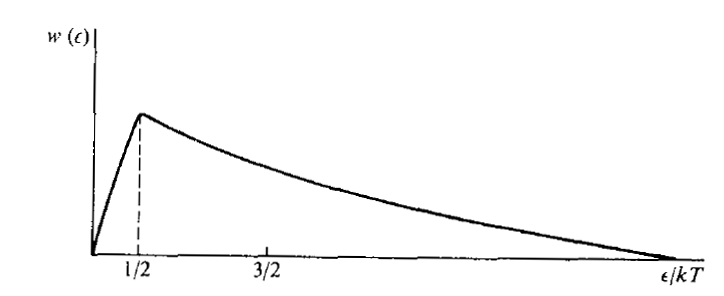
\includegraphics[width=0.6\textwidth]{Immagini/Edistr1.png}
		\caption{}
		\label{fig:Edistr1}
\end{figure}
Si riporta in \cref{fig:Edistr1,fig:EdistrN} la forma delle distribuzioni di probabilità in energia per una particella e per $N \gg 1$.
\newline

Per capire meglio il comportamento delle fluttuazioni in esame si studia il modello di gas ideale, per cui:
\begin{align*}
E &= \bar{\mathcal{E}} = \frac{3}{2} N k_B T\\
C_V &= \partdev{E}{T} = \frac{3}{2} N k_B
\end{align*}

\noindent Per cui si otttiene per le fluttuazioni relative:
\begin{equation*}
\frac{\sqrt{\overline{(\Delta E)^2}}}{E} = \frac{\sqrt{k_B T^2 \frac{3}{2}Nk_B}}{\frac{3}{2}Nk_B T} = \frac{\sqrt{N}}{N \sqrt{\frac{3}{2}}} \sim \frac{1}{\sqrt{N}}
\end{equation*}

\noindent e quindi vanno a $0$ per $N \rightarrow \infty$.

\begin{figure}[b!]
		\centering
		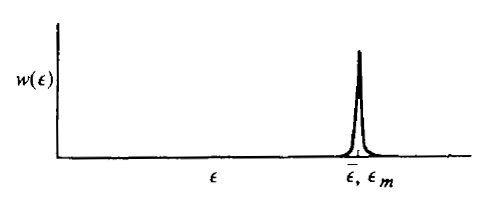
\includegraphics[width=0.6\textwidth]{Immagini/EdistrN.png}
		\caption{}
		\label{fig:EdistrN}
\end{figure}

\subsubsection{Fluttuazioni della densità}
Si possono studiare nello stesso modo le fluttuazioni della densità. Si prende quindi in esame il granpotenziale:
\begin{equation*}
\partfix{^2 \Omega}{\mu^2}{T,V} = \partdev{^2}{\mu^2} \left[ -k_B T \log \sum_{\alpha} \exp \left(- \frac{E_\alpha - \mu N_\alpha}{k_B T}\right)\right] = - \frac{1}{k_B T} (\overline{N_\alpha^2} - N^2)
\end{equation*}

\noindent cioè:
\begin{equation*}
\overline{(\Delta N)^2}(\overline{N_\alpha^2} - N^2) = - k_B T \partfix{^2 \Omega}{\mu^2}{T,V} = k_B T \partfix{N}{\mu}{T,V}
\end{equation*}

Inoltre, usando l'equazione di Gibbs-Duhem (vedi \cref{sec:thermquant}), si ottiene:
\begin{equation*}
\partfix{\mu}{N}{T,V} = \frac{V}{N} \partfix{P}{N}{T,V} = \frac{1}{N} \partfix{P}{\rho}{T,V}
\end{equation*}

\noindent dove $\rho = N/V$ è la densità. Ricordando or la definizione di compressibilità isoterma si ottiene:
\begin{equation*}
	K_T = - \frac{1}{V} \partfix{V}{P}{T} = - \rho \partfix{1/\rho}{P}{T} = \frac{1}{\rho} \partfix{\rho}{P}{T}
\end{equation*}

\noindent si trova infine il valore delle fluttuazioni in funzione di $N,T,\rho$:
\begin{equation*}
	\partfix{\mu}{N}{T,V} = \frac{1}{N \rho K_T} \qquad \implies \qquad \overline{(\Delta N)^2} = N k_B T \rho K_T
\end{equation*}

Si ottiene quindi per le fluttuazioni relative:
\begin{equation*}
	\frac{\overline{(\Delta V)^2}}{V^2} = \frac{\overline{(\Delta N)^2}}{N^2} = \frac{kT\rho}{N} K_T = \frac{kT}{V} K_T
\end{equation*}

\noindent dove la prima uguaglianza è giustificata dal fatto che si stanno considerando fluttuazioni della densità.

Ancora una volta si prova il risultato ottenuto sul gas ideale:
\begin{align*}
PV &= Nk_B T\\
K_T = - \frac{1}{V} \partfix{V}{P}{T} &= \frac{N k_B T}{P^2 V} = \frac{1}{P}\\
\frac{\sqrt{\overline{(\Delta N)^2}}}{N} &= \frac{\sqrt{k_B T / PV}}{N} = \frac{1}{\sqrt{N}}
\end{align*}

\noindent cioè si è ottenuto ancora una volta che le fluttuazioni si annullano con $1/\sqrt{N}$ per $N \rightarrow \infty$.

\subsubsection{Fluttuazioni nelle altre grandezze}
Se la densità viene mantenuta fissa si ha che le fluttuazioni nelle altre osservabili termodinamiche sono determinate da quelle dell'energia.

\begin{es}[Fluttuazioni nella temperatura, a densità fissata]
	Si determinano quindi a partire dall'energia:
	\begin{align*}
		\Delta T &= \partfix{T}{E}{V,N} \Delta E = \frac{\Delta E}{C_V}\\
		\overline{(\Delta T)^2} = \frac{\overline{(\Delta E)^2}}{C_V^2} = \frac{k_B T^2}{C_V}
	\end{align*}
	valido finché la densità è mantenuta costante.
\end{es}

\noindent Se la densità non fosse costante anche le fluttuazioni nell'energia sarebbero differenti, a causa del contributo della densità.

